\newpage
\topskip0pt
\vspace*{\fill}
\section*{Abstract}
Trade-offs are considered an important driver of species richness, as trade-offs between life history traits allow for niche specialisation. Plant communities are thought to have three important life history traits; fecundity, juvenile growth and defence against herbivores and/or abiotic pressures. We build upon the model presented in Chapter~2 to consider a variety of trade-offs in an environment that experiences disturbance events of varying intensity and frequency. Using invasion analysis, we enumerate the likelihood of each of these trade-offs allowing to species to coexist, and find that trade-offs between all three traits are most likely to promote coexistence, although this trade-off does not exhibit a significantly greater likelihood of coexistence than a fecundity-growth trade-off. Further, we demonstrate that trade-offs involving growth rate differences are robust to changes in community size, while a fecundity-defence trade-off cannot sustain more than a single species in large communities. 
\vspace*{\fill}
\newpage

\section{Introduction}
No single species can allocate unlimited resources to each life history trait \citep{law1979optimal,tilman1982resource}. Instead, species life histories are determined by the allocation of limited resources to different areas of need. In plant species, the three important life history traits are reproduction, growth from seedling to adult, and defence against both herbivory and abiotic factors such as fire \citep{bazzaz1987allocating}. This leads to trade-offs between life history traits; for example, a species with high levels of resource allocated to increasing fecundity will not be able produce seeds of a large mass \citep{turnbull1999seed} and, \textbf{since seed size is positively correlated with juvenile growth rate, is therefore likely to} experience a decrease in its juvenile growth rate \citep{gross1984effects}, or a species with rapid growth may be more susceptible to damage by storm winds or other mortality pressures such as large scale herbivory \citep[e.g.][]{wright2010functional,fine2006growth}. Theory has shown that these trade-offs can allow two or more species to coexist while competing for  the same resources in an environment \citep[e.g.][]{kisdi2003coexistence,levins1971regional,bonsall2004life}, suggesting that trade-offs are important for sustaining high levels of biodiversity in nature. \textbf{However, while some studies have compared several trade-offs \citep[e.g.][]{tilman1990constraints,grime1977evidence}, little is understood about how multiple trade-offs combine to affect community diversity, and whether trade-offs on multiple axes increase diversity in an additive manner.}

However, conditions under which species coexist alongside others will also be dependent on other, abiotic factors. Several previous studies have suggested that disturbance events also play an important role in promoting and maintaining diversity \citep[e.g.][]{sousa1984role,denslow1987tropical}.  Recent theoretical work \citep[Chapter~1;][]{miller2011frequency,nattrass2012quantifying} shows that different measures of disturbance, such as frequency or intensity, will have very different effects, even when the total biomass lost to disturbance over a given time period is taken into account. While many empirical studies consider disturbance as a single parameter \citep[e.g.][]{molino2001tree,peterson1997tornado,nakagawa2000impact}, some studies do demonstrate that different factors determining disturbance can affect the community structure differently. \cite{hall2012diversity} use bacterial populations to experimentally demonstrate that the frequency and intensity of disturbance events have different impacts, while \cite{denslow1980patterns} indicates that communities with large, infrequent disturbances may be more diverse than those where disturbance events are more frequent, yet clear a smaller area (e.g. tree-fall gaps). 

Here, all possible trade-offs between the three important plant life history traits - reproduction, juvenile growth and defence - are considered in a two species model. Defence is taken here to mean the ability of an individual to withstand a disturbance event, that is, an event that results in the death of large number of individuals and alters niche opportunities within the community, while seed production (seed number per capita per year) is used as the measure of fecundity. We therefore consider 8 models. The model where all species are identical gives neutral dynamics, and the coexistence of the two species is governed by chance, while the three models where the species differ in a single trait (no trade-off) demonstrate competitive exclusion of the weaker species. When trade-offs are between two or more traits, the effects of system capacity and varied disturbance regimes  are considered, and we show that trade-offs between fecundity and growth, or growth and defence, can support two species for large system sizes, as can a three dimensional trade-off, although a fecundity-defence trade-off cannot. The probability of species disturbance defence parameters resulting in coexistence is calculated, and we demonstrate that a three dimensional trade-off gives the greatest likelihood of coexistence, an order of magnitude larger than that of a growth-defence trade-off. Species specific disturbance intensities are then linked to allow comparison between the three dimensional trade-off and a fecundity-growth trade-off, \textbf{allowing us to test whether increasing the number of trade-off axes has a significant effect on diversity. When disturbance affects all species equally, we show that if the more fecund of the two species has a slight advantage in defence against disturbance, the likelihood of coexistence is maximised, although this increase is marginal}.


\section{Models}
Here, we build on the model presented in Chapter 2, introducing a single extra factor; we allow species to differ in the level of resource they dedicate towards resistance to disturbance events, so an individual of species $i$ will experience a species specific probability of death during a disturbance $I_i$. The model is described in a non disturbance time  step by the following transition probabilities (where $n=N_1(t)$ and $N-n=N_2(t)$);
\begin{align}
\label{inc}P(\text{increase}(n))=&\frac{N-n}{N}\frac{s_1 n}{s_1 n +s_2(N-n-1)}\exp \left( -s_2 \frac{N-n-1}{N} x\right),\\
\label{dec}P(\text{decrease}(n))=&\frac{n}{N}\frac{s_2 (N-n)}{s_1 (n-1) +s_2(N-n)}  \\
& + \frac{n}{N}\frac{s_1 (n-1)}{s_1 (n-1) +s_2(N-n)}\left(1-\exp \left( -s_2 \frac{N-n}{N} x\right)\right), \notag \\
\label{stay}P(\text{stay}(n))=&1-P(\text{increase}(n))-P(\text{decrease}(n)).
\end{align}
where $s_i$ is the per capita annual seed production of species $i$, $N$ is the system capacity - the maximum number of adults that can be sustained by the environment, and $x=C(1/g_1 - 1/g_2)/2$ is a measure of growth rate differences (with $C$ canopy height and $g_i$ the sapling growth rate of species $i$).

During a disturbance event, each individual of species $i$ will die with probability $I_i$. If there are $d_i$ deaths of species $i$, then the total deaths is given by $d=\sum_i d_i$. Note that $d$ is now dependent on the species composition of the community when the disturbance strikes, as well as the inherent properties of the disturbance. The expected number of deaths is given by
\begin{equation}
\label{avdeaths} \bar{d}=\sum_i I_i N_i(t)
\end{equation}
where $N_i(t)$ is the population of species $i$ at time $t$. Once all $d$ deaths occur, the remaining $N-d$ individuals compete for the opened sites in the system. If the populations of the two species are given by $n_1^*,n_2^*$ in the immediate aftermath of a disturbance, the probability of each gap being successfully colonised by species one is given by
\begin{equation}
\label{sp1c3}
Sp_1(n_1^*,n_2^*)=\frac{s_1 n_1^*}{s_1n_1^*+s_2n_2^*}\exp \left(-s_2 x\frac{n_2^*}{N}\right).
\end{equation}

We assess coexistence by considering invasion analysis. The average or expected change in a time step is approximated by
\begin{align}
\label{ac}
\text{AverageChange}(n)=&(1-f)\left(P(\text{increase}(n))-P(\text{decrease}(n))\right)  \\
&+f\left(-nI_1 +(nI_1+(N-n)I_2)Sp_1(n(1-I_1),(N-n)(1-I_2))\right).\notag
\end{align}
\textbf{This approximation does not account for Jensen's inequality, yet }Appendix~\ref{appapproximations} shows that for each of the models considered, the approximation \textbf{at the boundaries $(n=1,N-1)$} improves with system capacity $N$, and fits the actual expected change well. Coexistence occurs when on average, both species increase when rare; that is when
\begin{align}
\label{avch1}\text{AverageChange}(1)&>0,\\
\label{avchn-1}\text{AverageChange}(N-1)&<0. \end{align}

We can now consider a collection of models by varying different combinations of the three traits; fecundity, juvenile growth rate and defence or resistance to disturbance\textbf{, using the parameter values shown in Table~\ref{tabparas}.} This gives a selection of 8 models, one where the species are identical, 3 where they differ in a single parameter, 3 where they differ in two ways and the third parameter is equal, and a final model where species can differ in all three ways. The first four of these are trivial to analyse, but the models where species differ in at least two of the life history parameters give more interesting results.

\begin{table}[htdp]
\begin{center}
\begin{tabular}{|c|l|c|} \hline
\multicolumn{3}{|c|}{Table of baseline parameters} \\ \hline
Parameter & Description & Default value \\ \hline
$s_1$ & per capita annual seed production of species 1 & 500 \\ \hline
$s_2$ & per capita annual seed production of species 2 & 50\\ \hline
$g_1$&growth rate of species 1 juveniles & 13 \\
&(measured in mm/yr for diameter at breast height) &\\ \hline
$g_2$&growth rate of species 2 juveniles & 13.21 \\
&(measured in mm/yr for diameter at breast height) &\\ \hline
$C$& size of individuals at canopy height & 100 \\
& (measured in mm for diameter at breast height&\\ \hline
$x$&$C(1/g_1-1/g_2)/2$&0.06\\
&time window (yrs) for successful secondary colonisation by species 2&\\ \hline
$N$ & system capacity: number of individuals the region can support & 1000 \\ \hline
$n$ & number of species 1 individuals & N/A \\ \hline
$T_D$& average time between disturbances in yrs & 10 \\ \hline
$f$& within event disturbance probability & $100/(T_D N)$ \\ \hline
$I_1$& intensity of disturbance for species 1 & N/A \\ \hline
$I_2$& intensity of disturbance for species 2 & N/A \\ \hline
$y$ &Parameter linking species intensities; given by $I_1/I_2$ & N/A \\ \hline
\end{tabular} \end{center}
\caption{The key parameters used in the model, along with default values where appropriate}
\label{tabparas} 
\end{table}

\section{results}
When all species are identical, the model is simply a one-dimensional random walk, where disturbance events of intensity $I$ merely increase the distance it is possible to travel in a single step. Coexistence in this model is merely a function of chance. \textbf{This model therefore acts as a neutral theory model without mutation or speciation, where all species are equivalent and chance alone drives dynamics.} If the species merely differ in a single parameter, then we find that the species with the higher growth rate or fecundity, or with the lower mortality in a disturbance regime will competitively exclude the other.

\subsection{Fecundity-growth trade-off}
The case where species differ in both fecundity and growth ($I=I_1=I_2$) is analysed in detail in Chapter 2. In summary, for sufficiently low growth rate differentials $x$,  the more fecund species 1 can competitively exclude the rapidly growing species 2, both in the presence of disturbance and in an environment without disturbance. For intermediate $x$, coexistence is possible in the homogeneous environment, and this behaviour persists for low intensity or low frequency disturbances. As disturbance intensity increases (providing the frequency $f$ is greater than the expected time to extinction $t_{extinct}$), the fecundity advantage of species 1 will lead to it competitively excluding species 2. Thus, disturbance can lead to a decrease in diversity. When $x>x_{max}$ is large, species 2 will exclude the more fecund species 1 due to its superior growth rate. In this case, disturbance has a more complex effect. For frequencies $f$ such that $1/f > t_{extinct}$, intermediate disturbances will lead to coexistence of two species, while high intensities will allow the previously excluded species 1 to claim all sites and exclude species 2. Low intensities are insufficient to change the temporally homogeneous diversity, although may extend the time to coexistence. When $1/f < t_{extinct}$, species 2 will persist in monoculture. System size impacts the region of coexistence by increasing $t_{extinct}$, extending the region of more complex behaviour.

For a large system, or disturbances more frequent that $t_{extinct}$, the range of intensities that can give coexistence varies with the growth rate differential $x$, and is maximised at $x=x_{max}$, and also with the difference in fecundities. As seed numbers are varied, the maximum range of disturbance is at the point $s_1=s_2\exp(s_2x)$. That is, the range is maximised when the function $I=1-\ln(s_1/s_2)/(s_2x)$, formed by setting $\text{AverageChange}(1)=0$, returns $I=0$.

\subsection{Fecundity-defence trade-off}
When species have identical growth rates ($x=0$), yet differ in disturbance response and fecundities $s_i$, it is possible to find analytically the range of $I_1 - I_2$ space that gives coexistence for given fecundities $s_i$.\textbf{ We define $A(n)=(1-f)(P(\text{increase}(n))-P(\text{decrease}(n)))$, which is independent of $I_2$.} Setting $\text{AverageChange}(1)=0$ and solving for $I_1$ gives
\begin{align}
\label{fdac1sol}
I_1=&\frac{I_2(f(N-1)s_1-A(1)s_2(N-1)) +A(1)(s_1+s_2(N-1))}{I_2f(N-1)(s_1-s_2) +fs_2(N-1) +A(1)s_1}\notag \\
=&\frac{\alpha_1 I_2 +\beta_1}{\gamma_1 I_2+\delta_1}
\end{align}
while setting $\text{AverageChange}(N-1)=0$ gives the curve
\begin{align}
\label{fdacnsol}
I_1=&\frac{I_2(f(N-1)s_1-A(N-1)s_2) +A(N-1)(s_1(N-1)+s_2)}{I_2f(N-1)(s_1-s_2) +fs_2(N-1) +A(N-1)s_1(N-1)}\notag \\
=&\frac{\alpha_{N-1} I_2 +\beta_{N-1}}{\gamma_{N-1} I_2+\delta_{N-1}}
\end{align}
where
\begin{align}
\alpha_i =& f(N-1)s_1 - A(i) s_2 (N-i), \notag \\
\beta_i =& A(i) (s_1 i + s_2(N-i)), \notag \\
\gamma_i =& f(N-1)(s_1-s_2), \notag \\
\delta_i =& fs_2(N-1) + A(i)s_1 i. \notag
\end{align}
The region of coexistence is therefore the area between the two curves, as demonstrated in Figure~\ref{fd}(a). By noting that the indefinite integral of $(a x +b)/(c x +d)$ is $ax/c+(bc-ad)\ln(d+cx)/c^2 +const.$, we can write a formula for the area of the region of $I-$space that predicts coexistence;
\begin{align}
&\min \left(1, \int_0^1 dI_2 \quad \frac{\alpha_1 I_2 +\beta_1}{\gamma_1 I_2+\delta_1} \right) -  \int_0^1 dI_2\quad \frac{\alpha_{N-1} I_2 +\beta_{N-1}}{\gamma_{N-1} I_2+\delta_{N-1}}  \notag \\
=&\min\left(1,\frac{\alpha_1}{\gamma_1}+\frac{(\beta_1 \gamma_1 - \alpha_1 \delta_1)(\ln(\delta_1 +\gamma_1)-\ln(\delta_1)}{\gamma_1^2}\right) \\
&-\frac{\alpha_{N-1}}{\gamma_{N-1}}-\frac{(\beta_{N-1} \gamma_{N-1} - \alpha_{N-1} \delta_{N-1})(\ln(\delta_{N-1} +\gamma_{N-1})-\ln(\delta_{N-1})}{\gamma_{N-1}^2}. \notag
\end{align}
The minimum is taken in the first term because for sufficiently large $s_1$, the function given by \eqref{fdac1sol} is greater than one for all $I_2 \in (0,1)$, but an intensity of greater than 1 is impossible.\textbf{When
\begin{equation}
\label{fdto:lbint}
\int_0^1 dI_2 \quad \frac{\alpha_1 I_2 +\beta_1}{\gamma_1 I_2+\delta_1} >1
\end{equation}
the inequality $\text{AverageChange}(1)=0$ is satisfied for all possible combinations of disturbance defence parameters $I_1,I_2$. Therefore, the area of the region of $I-$space satisfying {avch1} is equal to the size of the whole region, 1. This minimum is not necessary in the second term, as the integrand
$$
\frac{\alpha_{N-1} I_2 +\beta_{N-1}}{\gamma_{N-1} I_2+\delta_{N-1}}
$$
tends to one from below as $s_1$ increases.}
 Hence, the region of coexistence does not change with $s_1$ in a smooth manner, as shown in Figure~\ref{fd}(d). The peak range of coexistence is given by intermediate $s_1=14225$ (for fixed $s_2=50$), with the region area tending to zero as the difference in species fecundities tends to infinity. For the chosen parameters, and system size $N=1000$, the peak probability of coexistence (when intensities for the two species are chosen at random) is approximately 0.120.
\begin{figure}[htbp]
\begin{tabular}{cccc}
(a)&&(b)&\\
&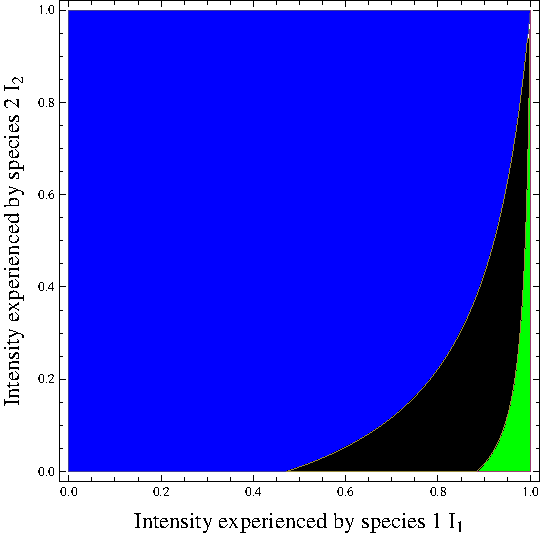
\includegraphics[width=2in]{fdtoexample.pdf}&&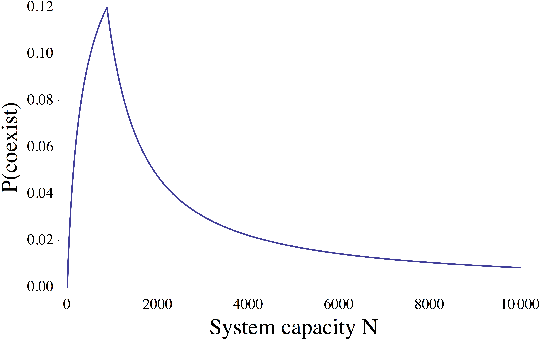
\includegraphics[width=2in]{fdtointwN.pdf} \\
(c)&&(d)&\\
&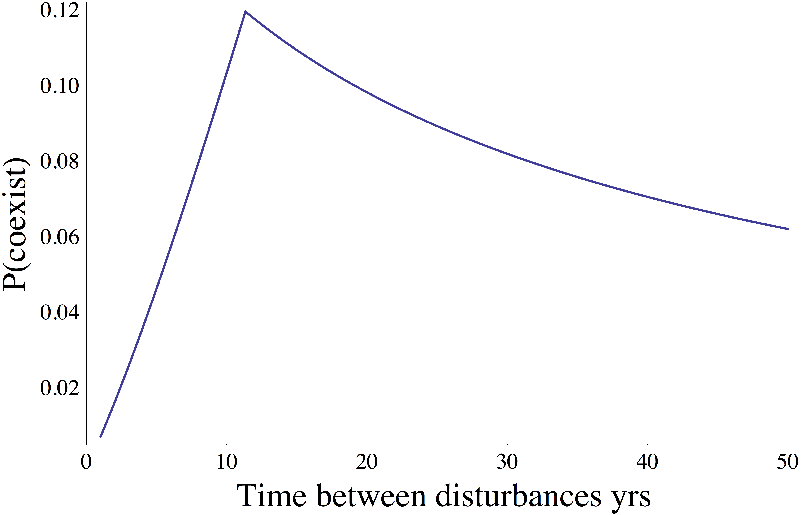
\includegraphics[width=2in]{fdtointwTd.pdf}&&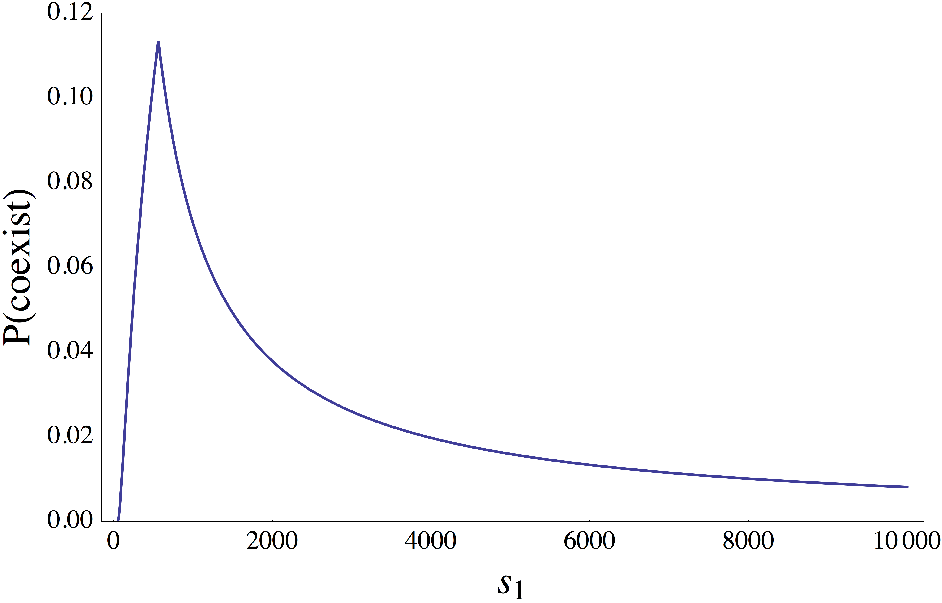
\includegraphics[width=2in]{fdtointws1.pdf}
\end{tabular}
\caption[Consequences of a fecundity-defence trade-off]{\textbf{Fecundity-defence trade-off:} (a) An example of the region of coexistence. The blue area (top and left, dark shading) is where species 1 can invade when rare, while the green area (bottom and right, pale shading) gives the region where species 2 can invade. The region where they overlap (black) is the region that gives coexistence. (b) The effects of changing system capacity on the area of the region of $I-$space that predicts coexistence. The region of coexistence peaks in area at intermediate system capacity $N\approx 850$, and declines with system size above this value. (c) The change in the likelihood of coexistence as time between disturbances $T_D$ is increased. The size of this region is maximised at intermediate values of $T_D \approx 10$, and tends to 0 as $T_D$ goes to infinity. (d) The change in the likelihood of coexistence as $s_1$ is increased. Note the discontinuity where \eqref{fdac1sol} becomes greater than one as $s_1=14225$.  Parameters $s_1=500,s_2=50,N=1000,T_D=10$ unless specified.}
\label{fd}
\end{figure}

Increasing frequency by reducing the expected time between disturbances $T_D$ also has a dramatic effect on the results. For very low frequency, \textbf{all combinations of defence responses exclude species 2, as the fecundity disadvantage it experiences cannot be overcome}. As frequency is increased, then very high $I_1$ can combine with low $I_2$ to give a small region of coexistence. For example, if a species devotes a great deal of resource to surviving fire, it could persist with a species very susceptible to fire but with a greater fecundity. \textbf{This advantage in fecundity ensures the species is better able to reach empty sites after a disturbance, and is therefore likely to claim sites uncontested by the poorer coloniser.} The range of parameters $I_i$ that give coexistence in this way increases with frequency until a threshold is reached (see Figure~\ref{fd}(c)) at which point, it is possible for species 2 to outcompete species 1 if $I_2<<I_1$.

The region of $I-$ space then begins to decline in area, \textbf{as the two curves comprising the boundaries of the region both tend to} the curve $I_1=I_2s_1/(I_2s_1+s_2(1-I_2))$ \textbf{as frequency $f$ tends to one ($T_D \to 0$).} In the limit as $f \to 1$ where `disturbance' events are so frequent as to provide an homogeneous environment themselves, both functions given by \eqref{fdac1sol} and \eqref{fdacnsol} are defined by this single curve, and coexistence is not possible. If $I_1>I_2s_1/(I_2s_1+s_2(1-I_2))$ then species 2 will dominate the environment, while if $I_1<I_2s_1/(I_2s_1+s_2(1-I_2))$ species 1 will exclude the less fecund species 2.

As system capacity $N$ increases, the range of coexistence shows a peak at $N \approx 850$. For wood or forest sized systems above this value, the region area will decline rapidly with increased system capacity. When the system capacity tends to infinity, the region of $I-$space giving coexistence tends to zero. A fecundity-defence trade-off cannot sustain two species in a large system, and has little effect in promoting biodiversity when system size reaches that of a forest or wood. The maximal effect on coexistence is restricted to a very small range of parameters, with steep declines in the probability of coexistence when moving away from these optimal parameter values. 

\subsection{Growth-defence trade-off}
A growth-defence trade-off ($s=s_1=s_2=50$) responds to changes in system capacity and frequency in a very different manner to the fecundity-defence trade-off outlined above. Here frequency has little effect provided that $1/f<t_{extinct}$, while if this condition is not satisfied, the faster growing species will exclude its competitor for any disturbance intensity regime. The response to system size is similar to that of the fecundity-growth trade-off\textbf{: as system capacity increases, the system asymptotes to a fixed region where coexistence is predicted.} Setting $\text{AverageChange}(1)=0$ and $\text{AverageChange}(N-1)=0$ gives $I_1$ as quadratic functions of $I_2$, $LBR(I_2), UBR(I_2)$, outlined in Appendix~\ref{approots}.
\textbf{The solutions presented in Appendix~\ref{approots} are each of the form
$$
\frac{-b\pm \sqrt{b^2-4ac}}{2a}.
$$ 
However, we note that each equation has one solution greater than one for all of the wide range of $x_s$ considered here. The solution given by the positive square root in \eqref{lbr}, and that given by the negative square root in \eqref{ubr} are both above one for all parameters tested. Therefore, these roots do not affect the behaviour of the system. The dynamics of the model are therefore determined by the negative square root in \eqref{lbr} and the positive square root in \eqref{ubr}.}
\begin{figure}[htbp]
\begin{tabular}{cccc}
(a)&&(b)&\\
&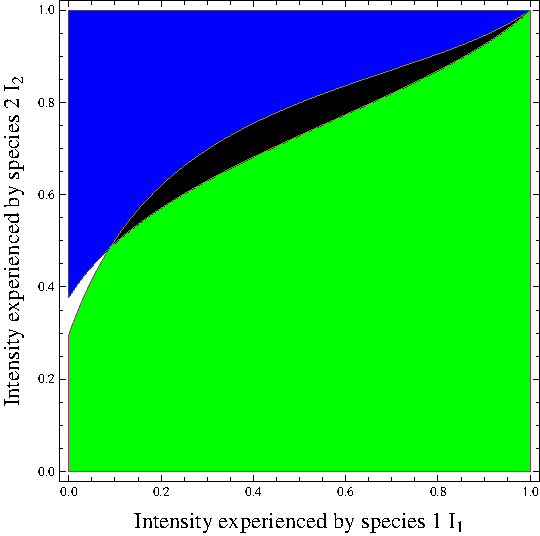
\includegraphics[width=2in]{gdx26.pdf}&&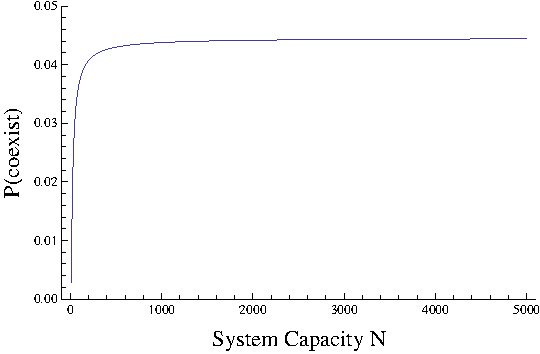
\includegraphics[width=2in]{gdtointwN} \\
(c)&&(d)&\\
&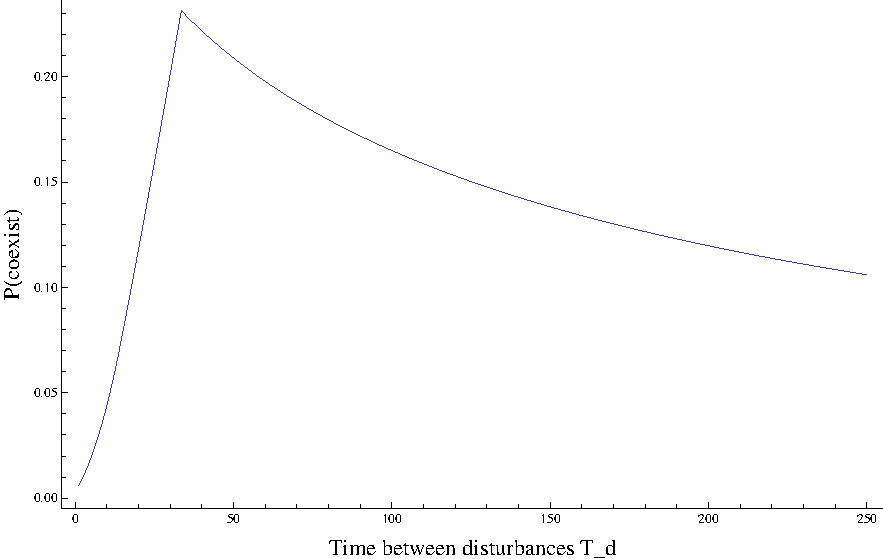
\includegraphics[width=2in]{gdtointwTd}&&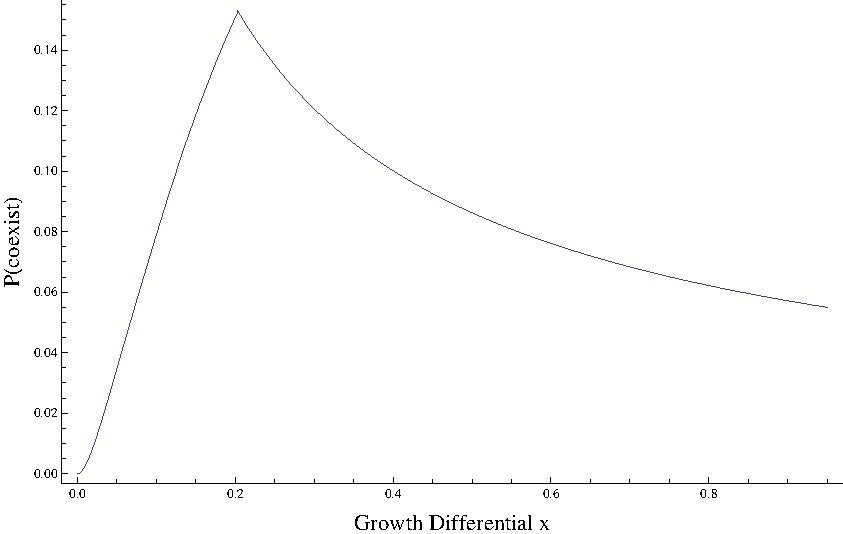
\includegraphics[width=2in]{gdtointwx}
\end{tabular}
\caption[Consequences of a growth-defence trade-off]{\textbf{Growth-defence trade-off:} (a) An example scenario, where coexistence can occur if both species suffer high mortality in a disturbance event. The blue area (top and left, dark shading) is where species 1 can invade when rare, while the green area (bottom and right, pale shading) gives the region where species 2 can invade. The region where they overlap (black) is the region that gives coexistence. The white region exhibits founder control. (b) The effects of changing system capacity $N$ on the likelihood of coexistence. As $N$ increases, the probability of coexistence stabilises as the integral asymptotes to a fixed value. (c) The change in the likelihood of coexistence as time between disturbances $T_D$ is increased. The size of this region is maximised at intermediate values of $T_D \approx 45$, and tends to 0 as $T_D$ goes to infinity. (d) The change in the likelihood of coexistence as $x$ is increased. Note the discontinuity where  the size of the region of coexistence peaks at $x\approx 0.2$. Parameters $s=50,x=0.06,N=1000,T_D=10$ unless specified.}
\label{gd}
\end{figure}

We can numerically integrate to find the area of the region of coexistence, using the following formula:
\begin{equation}
\int_{\max(0,I^*)}^1 dI_2\quad LBR(I_2) - \int_{\max(0,I^*)}^1 dI_2\quad UBR(I_2),
\end{equation}
where $I^*<1$ is the point at which $LBR(I^*)=UBR(I^*)$. \textbf{This point exists, and is unique, for all parameters tested, although confirming this uniqueness for any parameter choices is beyond the scope of the current work. Note that for all parameters, $LBR(1)=UBR(1)$.} This numerical integration allows us to study the behaviour of the system as $x$ is varied. When $x=0$ and the growth rates are identical, the species with the most resistance to disturbance (lowest $I_i$) will exclude its competitor.  As $x$ is increased, four distinct regions will occur, as in Figure~\ref{gd}(a). When both species display high resistance to disturbance (low $I_i$) there is a small region where neither $\text{AverageChange}(1)>0$ or $\text{AverageChange}(N-1)<0$ are satisfied, and founder control occurs, where coexistence does not occur and the successful species depends on the initial populations, subject to stochastic noise. When both species have higher intensities, there exists a region where coexistence is expected. Together the two regions of coexistence and founder control form a band from across $I-$space that separate regions where species and species 2 will exclude the other. We find the region of coexistence peaks at intermediate $x \approx 0.2$, when the probability of two species with randomised defence regimes coexisting is approximately $0.15$. As $x$ increases beyond this, the region of coexistence declines and tend to the region of $I-$space where $I_2>>I_1$, eventually tending to zero as $x$ tends to infinity.

\subsection{Three dimensional trade-off}
When species are allowed to vary in all three traits, fecundity, growth and defence, the region of coexistence is given by integrating the \textbf{functions \eqref{lbr} and \eqref{ubr}, as} determined in Appendix~\ref{approots}. For the three dimensional trade-off, this integral takes the form
\begin{equation}
\int_{\max(0,I^*,I^+)}^1 dI_2 \quad LBR(I_2) - \int_{\max(0,I^*,I^{++})}^1 dI_2 \quad UBR(I_2),
\end{equation}
where $LBR(I^*)=UBR(I^*)$ with $I^*<1$, $LBR(I^+)=0$, and $UBR(I^{++})=0$. \textbf{For all parameters considered here, these points are well defined and unique.} As in the growth-defence case, the roots with the negative square root are those that control the behaviour of the system. Numerically integrating, we can again calculate the region of coexistence in $I-$space. The region of coexistence in $I-$space is shown in Figure~\ref{full}(a). Calculating the areas of coexistence shows that for fixed seed numbers, the area of coexistence will peak at intermediate values of $x$, while for fixed $x$, the range of coexistence will increase as the discrepancy in fecundities becomes more pronounced. This increase will asymptote to the point where it is not possible for species 2 to exclude species 1, but where a significant proportional of trait space will give coexistence (See Figure~\ref{full}(d,f)). The region of coexistence generated by this model is consistently larger than that of the other two models (with $s_1=500,s_2=50,T_D=10,N=1000$, we see that the maximum range of coexistence is given when $x\approx 0.22$, and this region of coexistence has area $\approx 0.271$)
\begin{figure}[htbp]
\centering
\begin{tabular}{rrrr}
(a)&&(b)&\\
&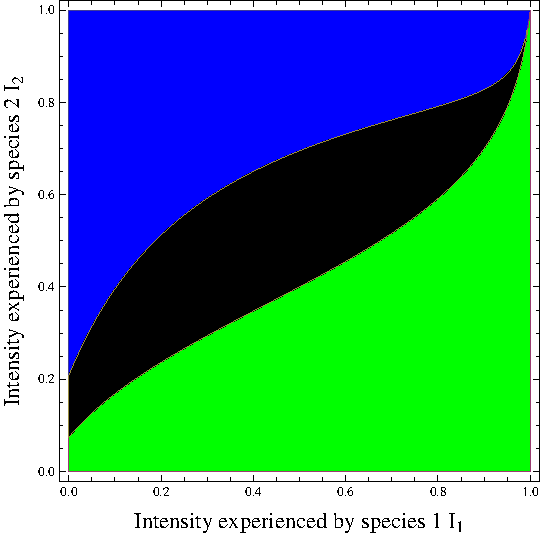
\includegraphics[width=2in]{fullexample.pdf}&&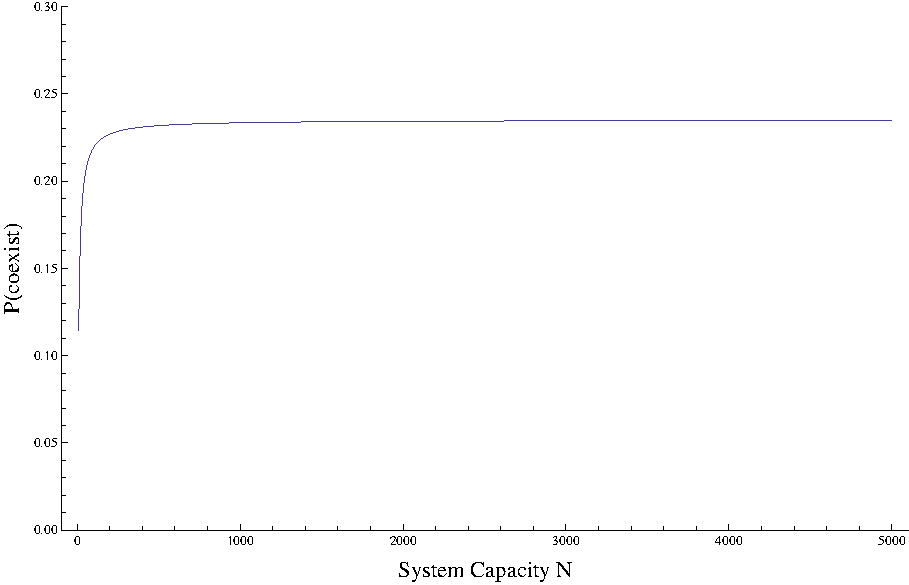
\includegraphics[width=2in]{fullintwithN.pdf} \\
(c)&&(d)&\\
&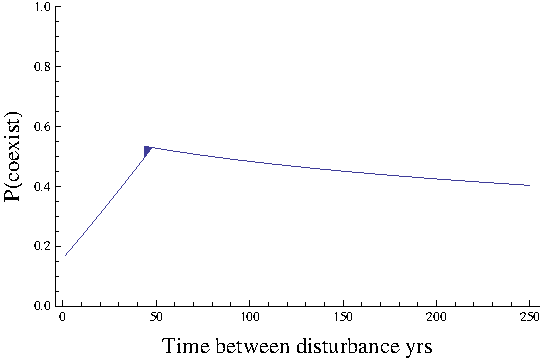
\includegraphics[width=2in]{fullintwTd.pdf}&&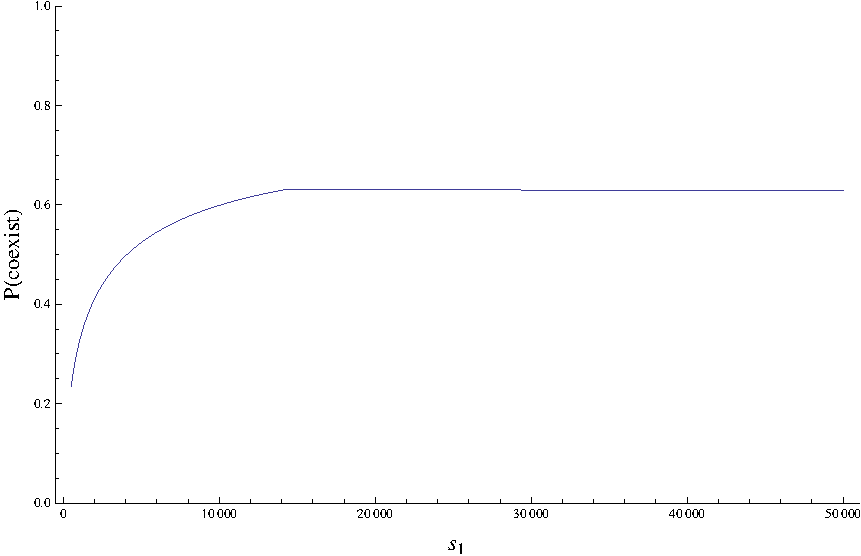
\includegraphics[width=2in]{fullintwiths1.pdf} \\
(e)&&(f)&\\
&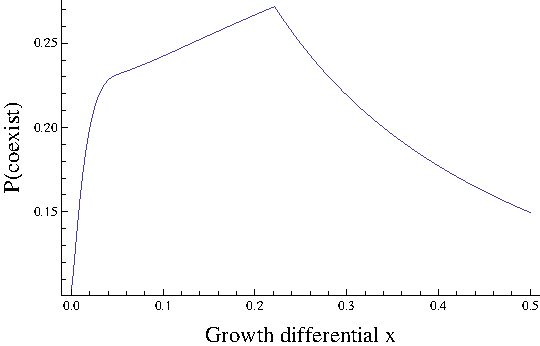
\includegraphics[width=2in]{fulltointwx.pdf}&&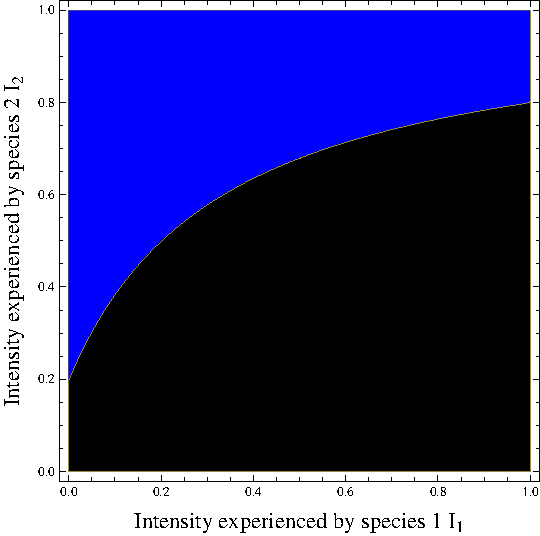
\includegraphics[width=2in]{fulllarges1.pdf}
\end{tabular}
\caption[Consequences of a three-dimensional trade-off]{\textbf{Three-dimensional trade-off:} (a) An example of $I-$space. The green/pale region to the bottom and right are where species 2 is dominant, while the blue/dark region (top and left) give species 1 monoculture. Where these regions overlap there is coexistence (black). (b),  (c) The change in the region of coexistence as $x$ varies, with a peak at intermediate values. (d) The size of the region given in (b) asymptotes as $s_1$ increases. Parameters $s_1=500,s_2=50,x=0.06,N=1000,T_D=10$ used to generate images unless specified. (e) The size of the region of coexistence and how it varies with $x$. The probability of coexistence increases rapidly with low $x$, and then experiences a slower increase for $0.046<x<0.22$. Above $x=0.22$ (f) When $s_1$ tends to infinity, a large proportion of $I-$space can support both species, although species 2 dominance is not possible ($s_1=10^6$).}
\label{full}
\end{figure}

\subsection{Linked intensities}
It is perhaps unrealistic to allow the responses to disturbance to \textbf{ be unconstrained within} $I-$space. Species specific responses are likely to be linked, such that as one increases, the other also increases. \textbf{For example, a tropical storm may cause only low level disturbance intensities that differ between species. These species may still differ should the tropical storm develop into a hurricane. However, we would anticipate that this escalation of disturbance pressure would serve to increase the intensity experienced by both species.} To simulate this, we consider the \textbf{simplest, linear,} case where $I_1=yI_2$, such that $y$ is a measure of the differences in the life history strategies of the two species, and $I_2$ is the force of a given disturbance event, normalised to the response of species 2. Note that for $y\neq 1$, one species will experience certain mortality while the other may retain some individuals.\textbf{ This occurs since when $I_2=1$, $I_1=y1=y\neq1$. Since $I_1$ is strictly increasing with $I_2$, when $0<y<1$ the intensity experienced by species one will be less than unity, $I_1<1$. Thus, while species 2 will go extinct in the next disturbance event, species 1 is expected to retain some of its population, and therefore colonise the entire community. Similarly, when $y>1$, when $I_2=1/y <1$, $I_1=1$ and species one will go extinct in the next disturbance, while species 2 can survive.} As intensity increases beyond this point, the two intensities will converge at one, but as the species with the lower resistance already experiences extinction, this will not affect the likelihood of species coexisting.

In the three dimensional trade-off model, we consider the effects of changing $y$ on the range of disturbances that can give coexistence for the parameters $s_1=500,s_2=50,x=0.06,T_D=0.5$.

We can then plot the average change at the boundary as a function of $I_2$ for differing $y$. We find dramatically different behaviour as $y$ varies. For $y$ sufficiently large ($y>1.39$ for the current parameters), so that species 2 has a huge advantage in survival of a disturbance event, we find that for all intensities, coexistence does not occur, and species 2 exists in monoculture. Here, the increased fecundity of species 1 is not sufficient to overcome the dual advantage of species 2, with its superior juvenile growth rate and increased resistance to disturbance, as shown in Figure~\ref{linked}(a).

\begin{figure}[htbp]
\begin{tabular}{rrrr}
(a)&&(b)&\\
&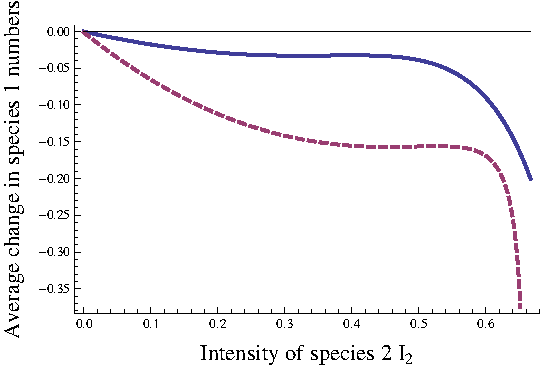
\includegraphics[width=2in]{highy.pdf}&&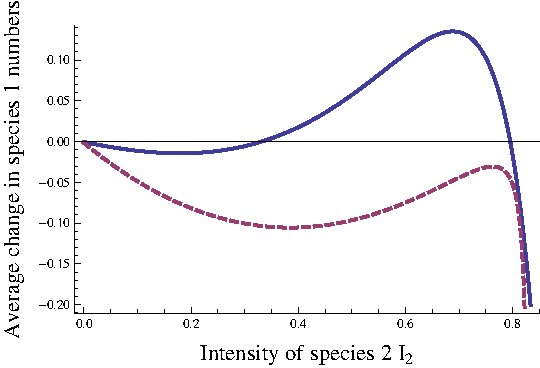
\includegraphics[width=2in]{lbworkubnot.pdf} \\
(c)&&(d)&\\
&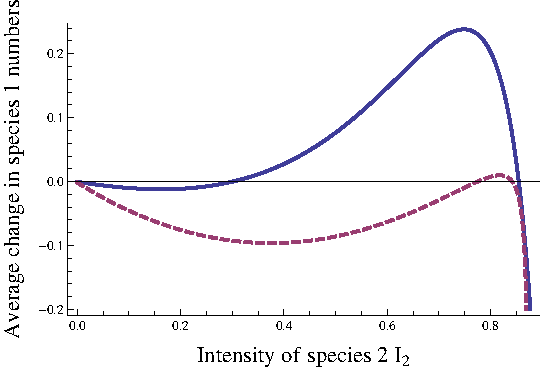
\includegraphics[width=2in]{fourbits.pdf}&&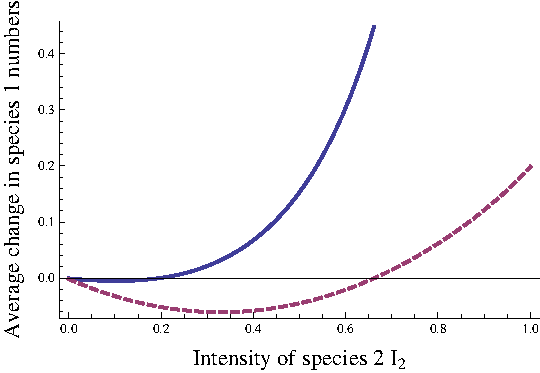
\includegraphics[width=2in]{onerooteach.pdf} \\
\end{tabular}
\caption[Effects of linking species specific disturbance intensities]{Plots of $\text{AverageChange}(1)$ (solid) and $\text{AverageChange}(N-1)$ (dashed) for different $y$. (a) $y=1.5$: $\text{AverageChange}(N-1)<1$ is satisfied for all intensities, but $\text{AverageChange}(1)>0$ never holds, so species 2 will exist in monoculture. (b) $y=1.2$:  $\text{AverageChange}(N-1)<1$ is satisfied for all intensities, but $\text{AverageChange}(1)>0$ holds for intermediate intensities. Therefore, coexistence will occur at intermediate intensities while at low and high intensities, species 2 will exist in monoculture. (c) $y=1.14$: Both curves have two real roots in the interval $[0,1]$, resulting in two bands of coexistence predicted by theory, with alternating monocultures surrounding them, species 2 monoculture at low and very high intensities, and species 1 at intermediate intensities. Note the higher band of predicted coexistence is not conformed by simulations, instead experiencing extinction of a random species due to the high intensity of disturbance events. (d) $y=0.9$: Both curves have a single real root in the interval $[0,1]$, resulting in a band of coexistence predicted by theory at intermediate intensity, with species 2 dominating at lower intensities while species 1 dominates at high intensities. $\text{AverageChange}(1)>\text{AverageChange}(N-1)$ for all $I_2$.}
\label{linked}
\end{figure}

As $y$ decreases, the behaviour then changes; $\text{AverageChange}(1)>0$ is satisfied for a range of intermediate disturbance intensities. At the same time, $\text{AverageChange}(N-1)$ remains below zero for all intensities $I_2$, meaning that coexistence is possible for intermediate intensities, but either side of this range species 2 will competitively exclude species 1 (Figure~\ref{linked}(b)). For the given parameters, the range of $y$ exhibiting this behaviour is approximately $1.16 \leq y \leq 1.38$. Decreasing $y$ further, making the two species response to disturbance more similar, \textbf{the behaviour of the system changes once more.} For $y\leq 1.15$, $\text{AverageChange}(N-1)$ has two real roots, and is positive between these roots. When $y>1$, both these roots occur in the interval $[0,1)$, as do two roots of $\text{AverageChange}(1)$. In this case, there are four distinct responses to disturbance as it increases in intensity (see Figure~\ref{linked}(c)). At low intensity, disturbance events are not strong enough to promote the more fecund species 1, so species 2 exists in monoculture. As intensity increases, then $\text{AverageChange}(1)>0$ is satisfied, while $\text{AverageChange}(N-1)<0$ continues to hold, giving coexistence of both species. Further increasing intensity, however, will result in $\text{AverageChange}(N-1)$ becoming positive. Here, species 2 will be competitively excluded, and species 1 will monopolise the system. Increasing intensity yet further results in $\text{AverageChange}(N-1)$ dropping back below zero, to give a secondary region where our invasion analysis predicts coexistence. However, for the parameters studied, the intensity here is high, and leaves a small remaining population (when $N=1000$, the remaining population is, on average, approximately 30 individuals). This reduced population is very susceptible to the stochasticity in the model, and all simulations result in one species going extinct by chance, although the identity of the surviving species varies between simulations. Increasing intensity even more, we have that $\text{AverageChange}(1)$ also drops below zero, so our theory predicts species two monoculture, which is once again matched by simulations, even given the extremely high intensities involved.

Once $y\leq 1$ there is only one root of $\text{AverageChange}(1)$ and one root of $\text{AverageChange}(N-1)$ in the interval $(0,1)$ (See Figure~\ref{linked}(d)). We therefore see a different type of behaviour again, with species 2 excluding the more fecund species 1 at low intensities, coexistence occurring at intermediate intensities, and species 1 excluding species 2 as high intensities.

As $y$ decreases towards zero, the range of intensities that can support both species will tend to a small interval, of width approximately $0.005$, at very low intensities ($0.005\lessapprox y \lessapprox 0.01$). We find that it is possible only to slightly increase the range of intensities giving coexistence from that of the case $y=1$, with $y=0.90$ (2 significant figures) giving a small increase in intensity range leading to coexistence. \textbf{The probability of species with randomly selected, yet linked, intensities coexisting with $y=0.9$ is given by $0.4666$, only slightly larger than the probability of coexistence when $y=1$, given by $0.4663$}, but this value declines again for $y<0.9$. That is, when the more fecund species 1 has a slight advantage in resistance to disturbance, the range of disturbances that the system can survive while maintaining its full biodiversity is maximised.

\section{Discussion}
Both life history trade-offs and disturbance events have been suggested as mechanisms that can promote and support high levels of diversity in nature. Here, we demonstrate that trade-offs among the three major life history traits for plants can give coexistence of at least two species competing within the same niche, and numerically quantify the likelihood of coexistence for each trade-off. However, the effectiveness of these trade-offs in supporting multiple species varies dramatically. Where species do not differ in juvenile growth rates, only small communities can possibly support more than a single species, and even in these small communities coexistence is extremely unlikely outside a very narrow range of parameters. This result suggests that a trade-off between seed production and resilience cannot realistically contribute to the diversity of a community, a view supported by the lack of empirical evidence in favour of this trade-off. \textbf{From the data in} \cite{martin2010dispersal}, \cite{martin2010divergence} concluded that ``it is unlikely that... survivorship come[s] at the expense of fecundity.'' While some other studies do find a correlation between \textbf{fecundity and defence} \citep[e.g.][]{marquis1984leaf,gwynn2005resistance} this relationship is often weak, suggesting that the selection pressure for such a trade-off is weak. We propose that \textbf{the limited} evidence for this trade-off is a consequence of other, more strongly selected trade-offs such as the growth-survival and fecundity-growth trade-offs.

Meanwhile, trade-offs between growth and either fecundity or disturbance resistance (or both) can support multiple species for any system capacity $N$. In a large system, we demonstrate that a trade-off involving all three of the major plant traits will give a probability of randomly selected disturbance resistances supporting two species higher than the probability given by a growth-defence trade-off alone. However, when species responses to disturbance are proportional (such that disturbance intensity for one species is doubled, the intensity for the second species is also doubled), the three dimensional trade-off does not significantly improve the likelihood of coexistence when compared to a fecundity-growth trade-off. These results suggest that the trade-off between fecundity and juvenile growth rate, or competition and colonisation, contributes much more to the maintenance of biodiversity than trade-offs involving disturbance resistance.  

\textbf{The current model only includes two species, although disturbance is also anticipated to enhance coexistence in multi-species communities \citep[e.g.][]{loehle2000strategy,roxburgh2004intermediate}. Theory has shown that infinitely many species may coexist along a competition-colonisation trade-off \citep{tilman1994competition,adler2000space}, although this coexistence is either highly unlikely or structurally unstable \citep{nattrass2012quantifying, gyllenberg2005impossibility}. In Chapter~4, the current model is extended to three species for the trade-off between fecundity and growth, while the model where species differ in all three traits is also considered. For tradeoffs between defence and either fecundity or growth, we anticipate qualitatively similar results for a multi species model, whereby a fecundity-defence trade-off will be extremely sensitive to changes in parameters, while a growth-defence trade-off is expected to be ore robust. A further extension of the model is to include spatial structure. While Chapter~4 again considers this in a simplified manner, a full spatial structure may have dramatic effects on coexistence, due to the propensity for species to show within-species clustering \citep{condit2000spatial,murrell2001uniting} and limitations on dispersal. As in the fecundity-growth model discussed in Chapter~2, we anticipate that spatial structure may assist the weaker competitor, as restricted dispersal may allow it to win sites by default.}

We conclude that a trade-off between fecundity, in the form of per capita annual seed production, and juvenile growth rates is more significant in sustaining biodiversity than trade-offs between growth and defence or fecundity and defence, and while species specific reactions to disturbance can slightly improve the likelihood of a fecundity-growth trade-off allowing two species coexistence, this increase is not significant. This concurs with empirical studies, which have found a great deal of support for a trade-off between fecundity and growth rate, or the equivalent competition-colonisation trade-off \citep[e.g.][]{levins1971regional,yu2001competition,tilman1994competition,adler2000space}. The high level of occurrence for this trade-off indicates that it has been an important driver in the evolution of those diverse communities, allowing two or more species to effectively occupy the same resource niche by the different allocation of that resource to their life history traits. That a trade-off between growth and defence can support some coexistence suggests that some support should be found for this trade-off in empirical studies, and this is indeed the case \citep[e.g.][]{wright2010functional,fine2006growth}. However, support for this is much less widespread than the fecundity-growth or competition-colonisation trade-off, which further supports our conclusion that the latter is the most significant driver of biodiversity.

\section*{Appendices}

\bappendix
 \section{Approximating the expected change function}
 \label{appapproximations}
 The expected change for the model when at the lower boundary $n=1$ is given by
 \begin{align}
\label{acreal1difi}&\text{AverageChangeReal}(1)=\frac{-I_1+(N-1)I_2^{N-1}(1-I_1)}{dNT_D}\\
&+\frac{(1-I_1)\sum_{k=1}^{N-2}\sum_{j=k}^{N-2}k I_2^j(1-I_2)^{N-2-j}{N-2\choose j} Sp_1(1,N-1-j)^k(1-Sp_1(1,N-1-j))^{j-k} {j \choose k}}{dNT_D} \notag \\
 &+ \left(1-\frac{1}{dNT_D}\right)(P(\text{Increase}(1))-P(\text{Decrease}(1))), \notag
 \end{align}
 while at the upper boundary $n=N-1$, the expected change is given by
\begin{align}
 \label{acrealtotdifi}&\text{AverageChangeReal}(N-1)= \frac{-I_1^{N-1}(N-1) +I_2(1-I_1^{N-1})}{dNT_D} \\
 &-\frac{(1-I_2)\sum_{k=1}^{N-2}\sum_{j=k}^{N-2}k I_1^j(1-I_1)^{N-2-j}{N-2\choose j} Sp_1(N-1-j,1)^{j-k}(1-Sp_1(N-1-j,1))^{k} {j \choose k}}{dNT_D} \notag \\
 &+ \left(1-\frac{1}{dNT_D}\right)(P(\text{Increase}(N-1))-P(\text{Decrease}(N-1))). \notag
  \end{align} 
These are approximated using \eqref{ac}. Figure~\ref{fig:fdtoapprox} shows how the size of the absolute error between the actual expected change and the approximation declines with system capacity $N$ for a trade-off between fecundity and defence ($x=0$), while Figures~\ref{fig:growthdefenceerrors} and \ref{fig:fullapprox} show that this result holds for the growth-defence trade-off ($s_1=s_2$) and the three dimensional trade-off respectively. The error was calculated for intensities $I=0.1,0.2,0.3,...,0.9$ and time between disturbances $\ln(T_D)=1,2,3,...,8,$, therefore giving 648 error values for each system size. The approximation is accurate even at relatively small $N>400$. While the results from only one set of parameters are shown, these results are robust to parameter changes.

   
   
 \section{Roots of average change for $x>0$}
 \label{approots}
 Using Mathematica 8.0.1.0 to set $\text{AverageChange}(1)=0$ and rearranging to solve for $I_1$ gives the solution
 \begin{small}
 \begin{align}
 \label{lbr}
&\frac{-e^{-\frac{(I_2-1) s_2 (N-1) x}{N}} }{200 s_1 N (s_1+s_2 (N-2)) e^{\frac{s_2
   (N-2) x}{N}} \left(e^{-\frac{(I_2-1) s_2
   (N-1) x}{N}}-1\right)}\times \\
&\begin{pmatrix}
\begin{matrix}
s_1^2   \left(-100 N (I_2 (N-1)-1) e^{\frac{s_2 x   (I_2 (N-1)-1)}{N}} \right. \\
   \left. +((T_D-100) N-100)   e^{\frac{s_2 (N-2) x}{N}}-(N-1) (T_D   N-100)\right) \\
   +s_1 s_2 \left(\left(N^2 (100   (I_2-2)+T_D)-2 N (50 (I_2-2)+T_D)+200\right)\right. \\
  \left. e^{\frac{s_2 (N-2) x}{N}}-100 (N-2)   N (I_2 (N-1)-1) e^{\frac{s_2 x (I_2   (N-1)-1)}{N}}\right)\\
   +100 (I_2-1) s_2^2   (N-2) (N-1) N e^{\frac{s_2 (N-2)   x}{N}}
   \end{matrix} \\
\pm \sqrt{ \splitfrac{e^{-\frac{2 (I_2-1) s_2 (N-1)  x}{N}}}
{\splitfrac{ \left(s_1^2 \left(-100 N (I_2   (N-1)-1) e^{\frac{s_2 x (I_2   (N-1)-1)}{N}}+((T_D-100) N-100)   e^{\frac{s_2 (N-2) x}{N}}\right. \right. }
{\splitfrac{\left. -(N-1) (T_D N-100)\right)+s_1 s_2 \left(\left(N^2 (100   (I_2-2)+T_D)-2 N (50 (I_2-2)+T_D)+200\right) \right.}
{\splitfrac{   \left. e^{\frac{s_2 (N-2) x}{N}}-100 (N-2)   N (I_2 (N-1)-1) e^{\frac{s_2 x (I_2   (N-1)-1)}{N}}\right)}
{\splitfrac{\left. +100 (I_2-1) s_2^2   (N-2) (N-1) N e^{\frac{s_2 (N-2)   x}{N}}\right)^2}
{\splitfrac{-400 s_1 N (s_1+s_2   (N-2)) e^{\frac{s_2 x (I_2 (-N)+I_2+2   N-3)}{N}} \left(e^{-\frac{(I_2-1) s_2   (N-1) x}{N}}-1\right) \times}
{\splitfrac{ \left(100 I_2 s_1   (N-1) N (s_1+s_2 (N-2))   e^{\frac{s_2 x (I_2 (N-1)-1)}{N}}\right.}
{\splitfrac{\left.-(T_D   N-100) (s_2 (I_2   (-N)+I_2+N-1)+s_1)\right.}{\left. \left((s_1+s_2   (N-2)) e^{\frac{s_2 (N-2) x}{N}}+s_1   (-N)+s_1\right)\right)}}}}}}}}} 
\end{pmatrix} \notag
   \end{align}
   \end{small}
 Similarly, the solution for $I_1$ when $\text{AverageChange}(N-1)=0$ is given by
 \begin{small}
 \begin{align}
 \label{ubr}
&UBR(I_2)=-\frac{e^{\frac{(3-2 I_2) s_2 x}{N}}}{N 200 s_1 (N-1)^2 (s_1 (N-2)+s_2)
   e^{\frac{s_2 x}{N}} \left(e^{-\frac{(I_2-1) s_2
   x}{N}}-1\right)}\times \\
& \begin{pmatrix}\splitfrac{\pm T_D N
   e^{\frac{(2 I_2-3) s_2 x}{N}} \times}{
   \begin{matrix}  \sqrt{ \frac{  \splitfrac{(N-1)^2
   \left(e^{\frac{2 (3-2 I_2) s_2 x}{N}} \times \right.}{\splitfrac{\left(s_1^2
   (N-2) (N-1) (T_D N-100)
   e^{\frac{(I_2-2) s_2 x}{N}}\right.}{\splitfrac{-(s_1
   (N-2)+s_2) e^{\frac{(I_2-1) s_2 x}{N}}}{\splitfrac{
   \left(100 (I_2-1) s_2 N+s_1 \left(T_D
   (N-2) N-100 \left(N^2-2\right)\right)\right)}{\splitfrac{\left. +100
   s_1 N (I_2-N+1) (s_1
   (N-2)+s_2) e^{\frac{2 (I_2-1) s_2
   x}{N}}\right)^2}{\splitfrac{-400 s_1 N (s_1
   (N-2)+s_2) e^{-\frac{2 (I_2-2) s_2 x}{N}} \times }
{\splitfrac{ \left(e^{-\frac{(I_2-1) s_2 x}{N}}-1\right)\times}{\splitfrac{ \left(s_1
   (N-2) (N-1) (T_D N-100) (-I_2
   s_2+s_1 (N-1)+s_2) e^{\frac{(I_2-2) s_2
   x}{N}}\right.}{\splitfrac{+(N-2) (T_D N-100) (s_1
   (N-2)+s_2) ((I_2-1) s_2+s_1
   (-N)+s_1) e^{\frac{(I_2-1) s_2 x}{N}}}{\left. \left.+100
   I_2 s_1 (N-1) N (s_1
   (N-2)+s_2) e^{\frac{2 (I_2-1) s_2
   x}{N}}\right)\right)}}}}}}}}}}
   {T_D^2 N^2}} \\
         +s_1^2   (N-2) (N-1)^2 (T_D N-100)   \left(-e^{\frac{(I_2-2) s_2 x}{N}}\right) \\
   +(N-1)   (s_1 (N-2)+s_2) \left(\left(100 (I_2-1) s_2   N\right. \right. \\
   \left.+s_1 \left((T_D-100) N^2-2 T_D   N+200\right)\right) \times \\
    \sinh \left(\frac{(I_2-1) s_2   x}{N}\right)\\
   +\left(100 (I_2-1) s_2 N+s_1   \left((T_D-100) N^2-2 T_D N+200\right)\right) \\
   \cosh \left(\frac{(I_2-1) s_2 x}{N}\right)+100 s_1   N (-I_2+N-1) \sinh \left(\frac{2 (I_2-1) s_2   x}{N}\right) \\
  \left.+100 s_1 N (-I_2+N-1) \cosh   \left(\frac{2 (I_2-1) s_2  x}{N}\right)\right)
   \end{matrix}} \end{pmatrix} \notag
  \end{align}

  \end{small}
 Note that for both the growth-defence trade-off, and the full three dimensional trade-off that also includes fecundity, one of the roots here is always above one. These roots are the positive square root for $LBR(I_2)$, and the negative root for $UBR(I_2)$. Therefore, the roots used to calculate the size of the region of coexistence are the negative and positive roots respectively.

 
   \begin{figure}[th]
\centering
   \begin{tabular}{rrrr}
   (a)&&(b)&\\
  &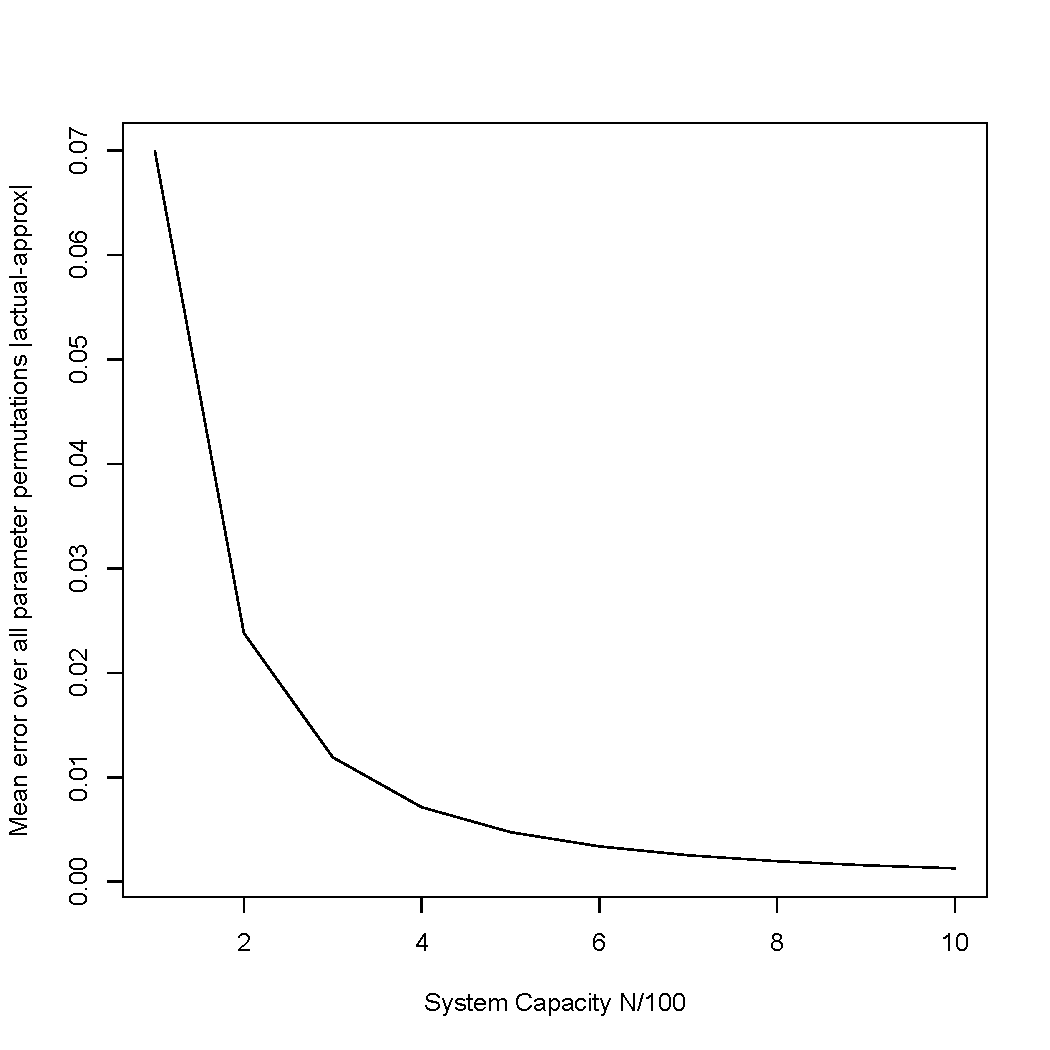
\includegraphics[width=2.5in]{FDmeanerr.pdf} && 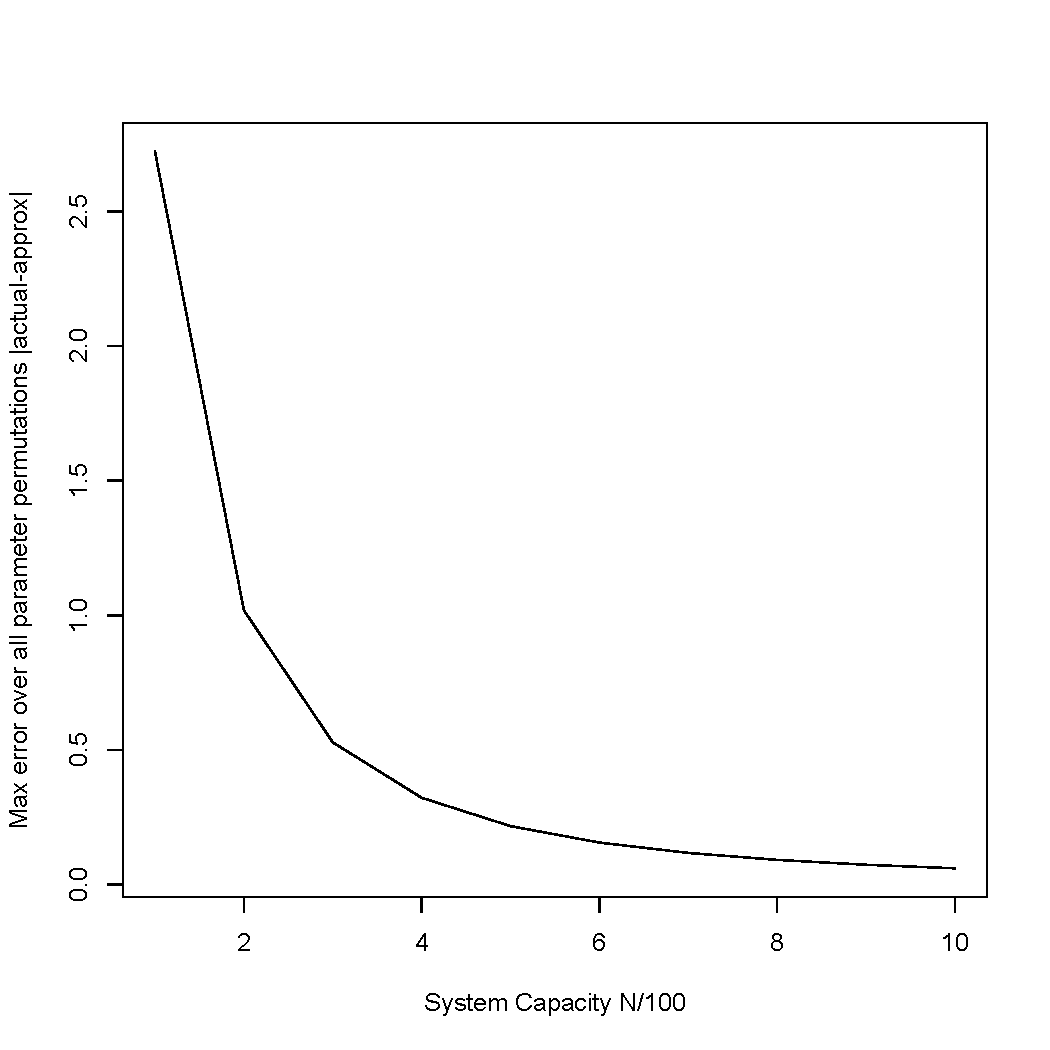
\includegraphics[width=2.5in]{FDmaxerr.pdf} \\
  (c)&&(d)&\\
  &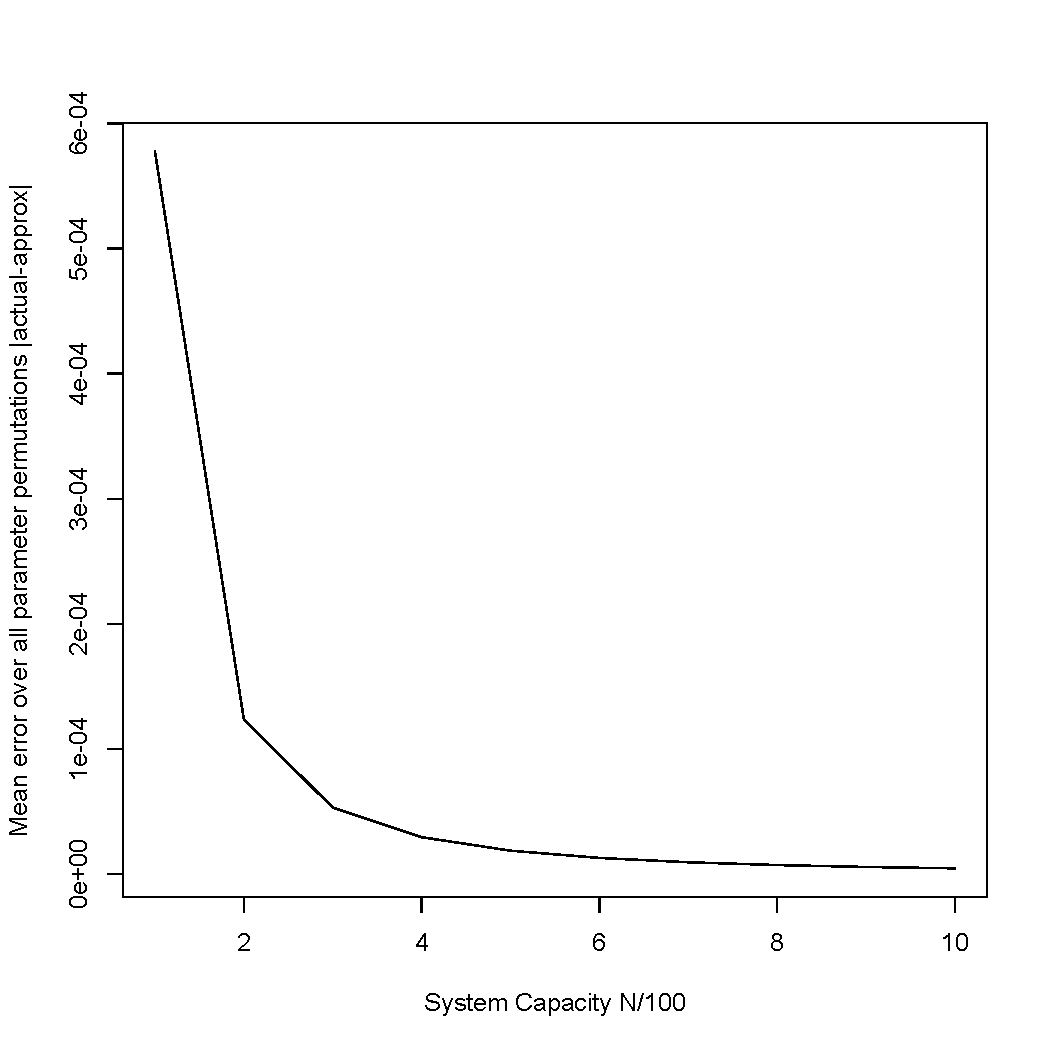
\includegraphics[width=2.5in]{FDtmeanerr.pdf} && 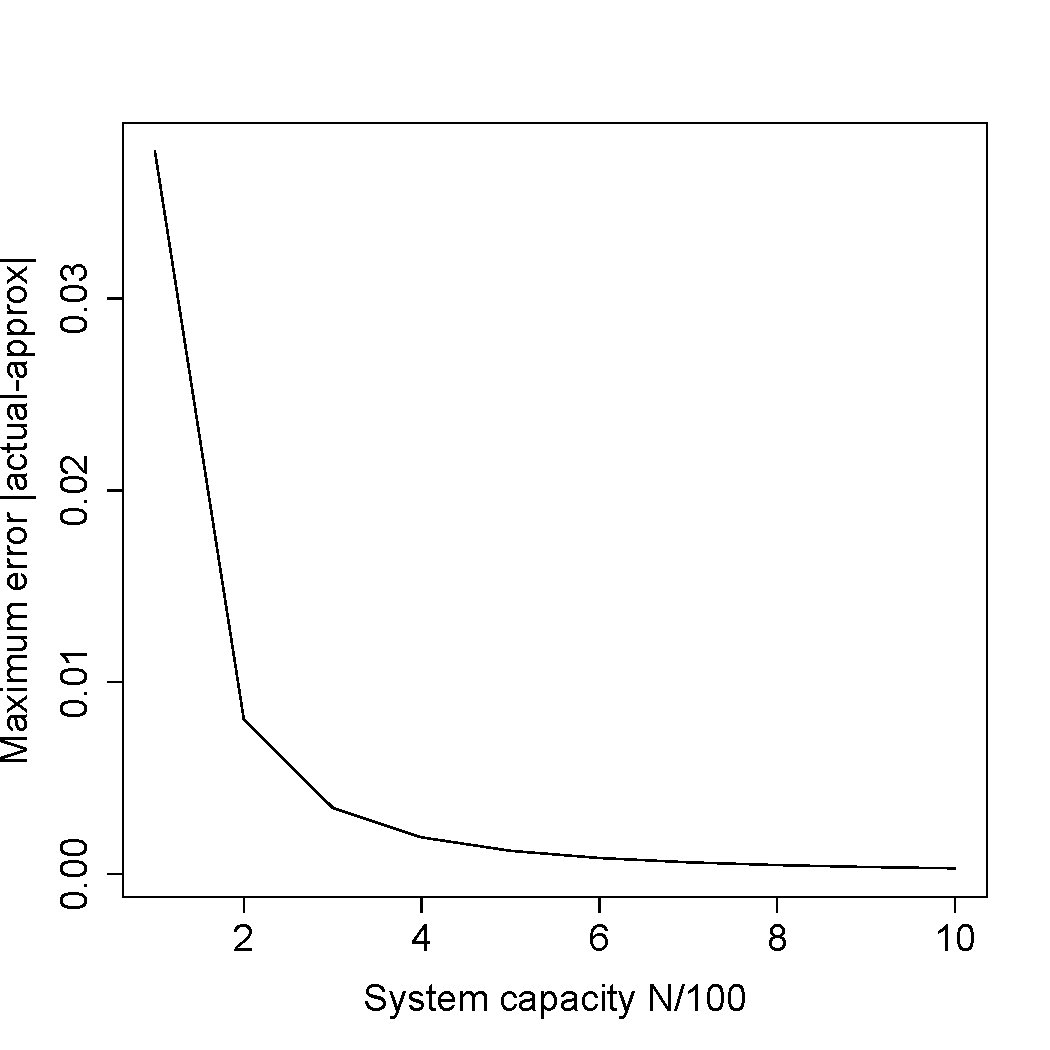
\includegraphics[width=2.5in]{FDtmaxerr.pdf} \end{tabular}
   \caption[Errors in approximating average change: fecundity-defence trade-off]{\textbf{Fecundity-defence trade-off:} (a-b)  How the mean (a) and maximum (b) error size at the lower boundary decrease with increased system capacity $N$. (c-d) How the mean (c) and maximum (d) error size at the upper boundary decrease with increased system capacity $N$. The error was calculated for intensities $I_1,I_2=0.1,0.2,0.3,...,0.9$ and time between disturbances $\ln(T_D)=1,2,3,...,8.$ Parameters used are $s_1=500,s_2=50$. Error is calculated as $| \text{AverageChangeReal}(n) - \text{AverageChange}(n) |$ for $n=1,N-1$.}
    \label{fig:fdtoapprox}
   \end{figure}
   
    \begin{figure}[th]
\centering
   \begin{tabular}{rrrr}
   (a)&&(b)&\\
  &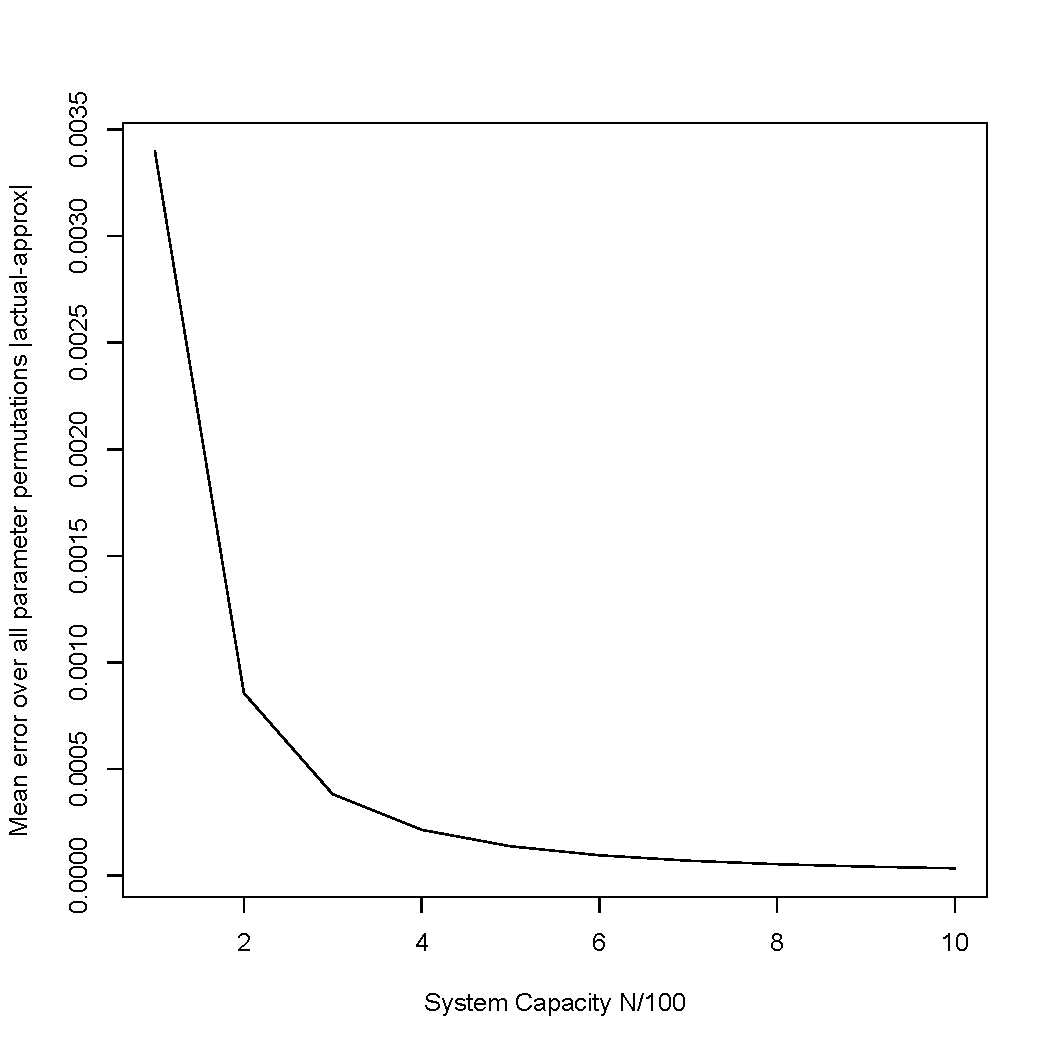
\includegraphics[width=2.5in]{GDmeanerr.pdf} && 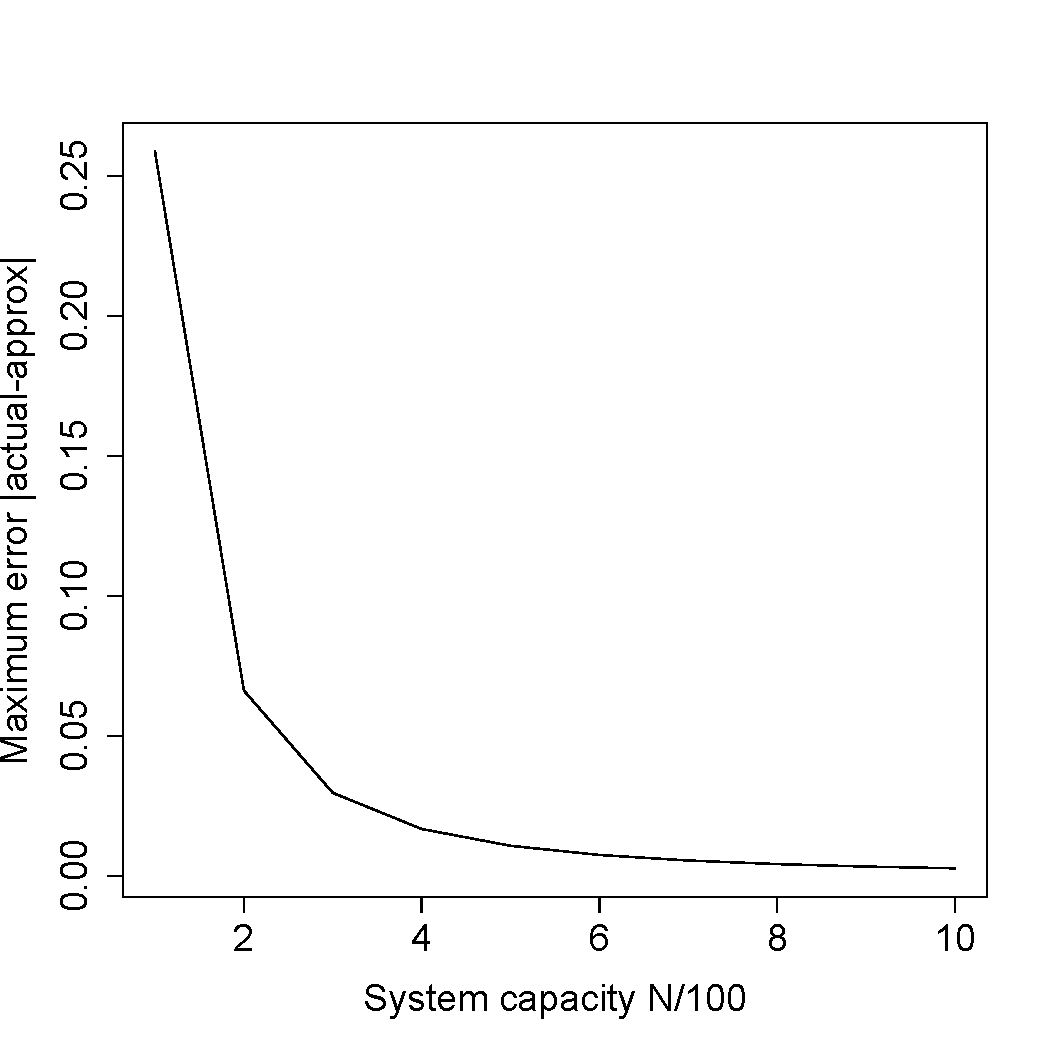
\includegraphics[width=2.5in]{GDmaxerr.pdf} \\
  (c)&&(d)&\\
  &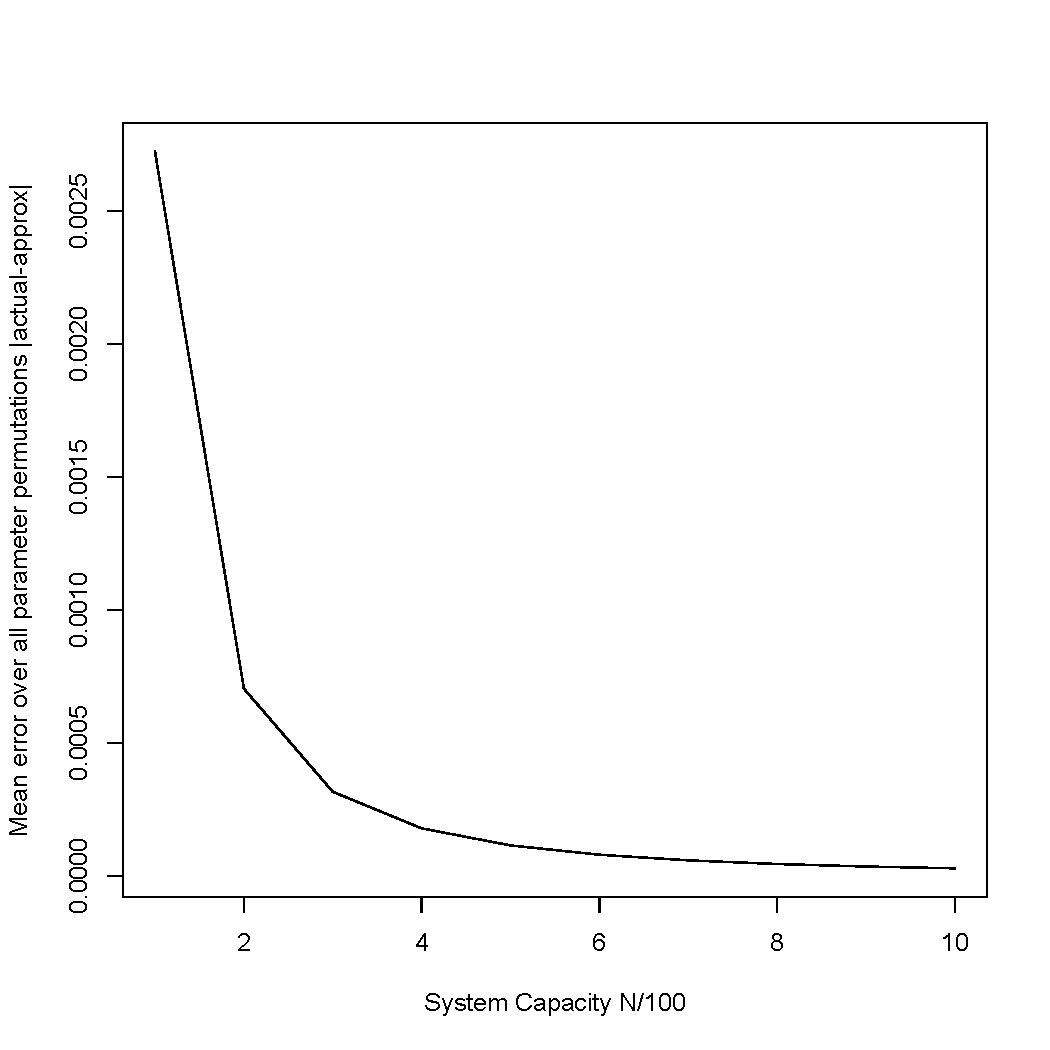
\includegraphics[width=2.5in]{GDtmeanerr.pdf} && 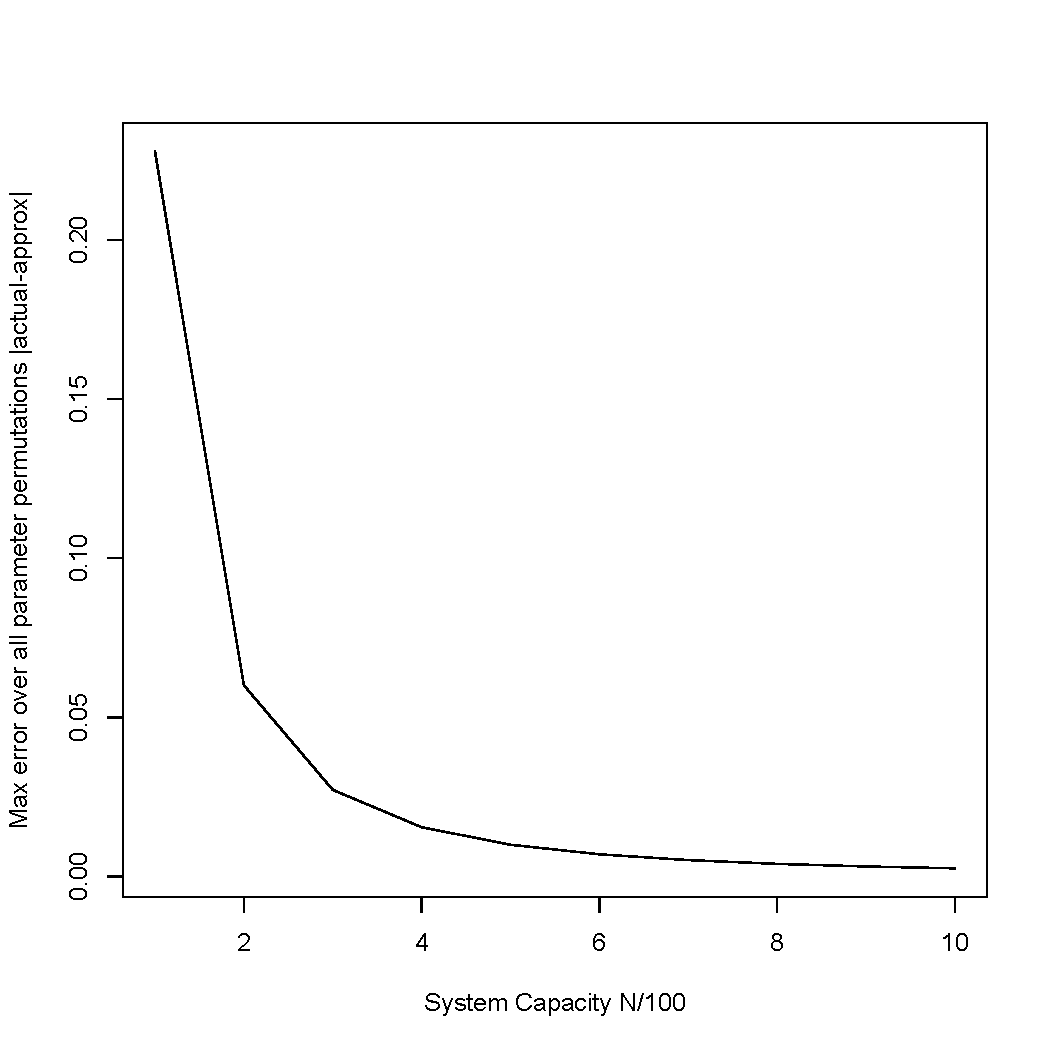
\includegraphics[width=2.5in]{GDtmaxerr.pdf} \end{tabular}
   \caption[Errors in approximating average change: growth-defence trade-off]{\textbf{Growth-defence trade-off:} (a-b)  How the mean (a) and maximum (b)  error size at the lower boundary decrease with increased system capacity $N$. (c-d) How the mean (c) and maximum (d) error size at the upper boundary decrease with increased system capacity $N$. The error was calculated for intensities $I_1,I_2=0.1,0.2,0.3,...,0.9$ and time between disturbances $\ln(T_D)=1,2,3,...,8.$ Parameters used are $s_1=50,s_2=50,x=0.06$. Error is calculated as $| \text{AverageChangeReal}(n) - \text{AverageChange}(n) |$ for $n=1,N-1$.}
     \label{fig:growthdefenceerrors}
    \end{figure}
    
     \begin{figure}[th]
\centering
   \begin{tabular}{rrrr}
   (a)&&(b)&\\
  &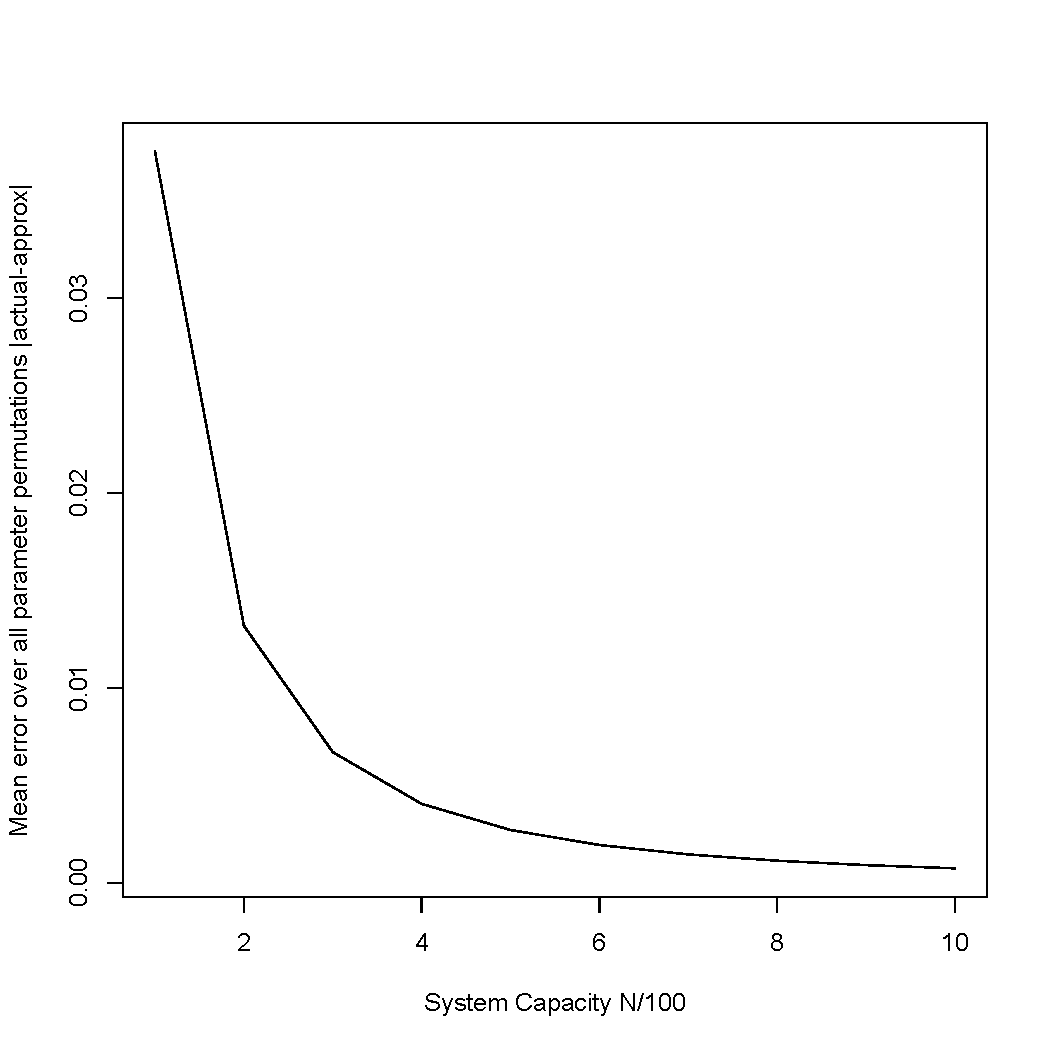
\includegraphics[width=2.5in]{FDGmearerr.pdf} && 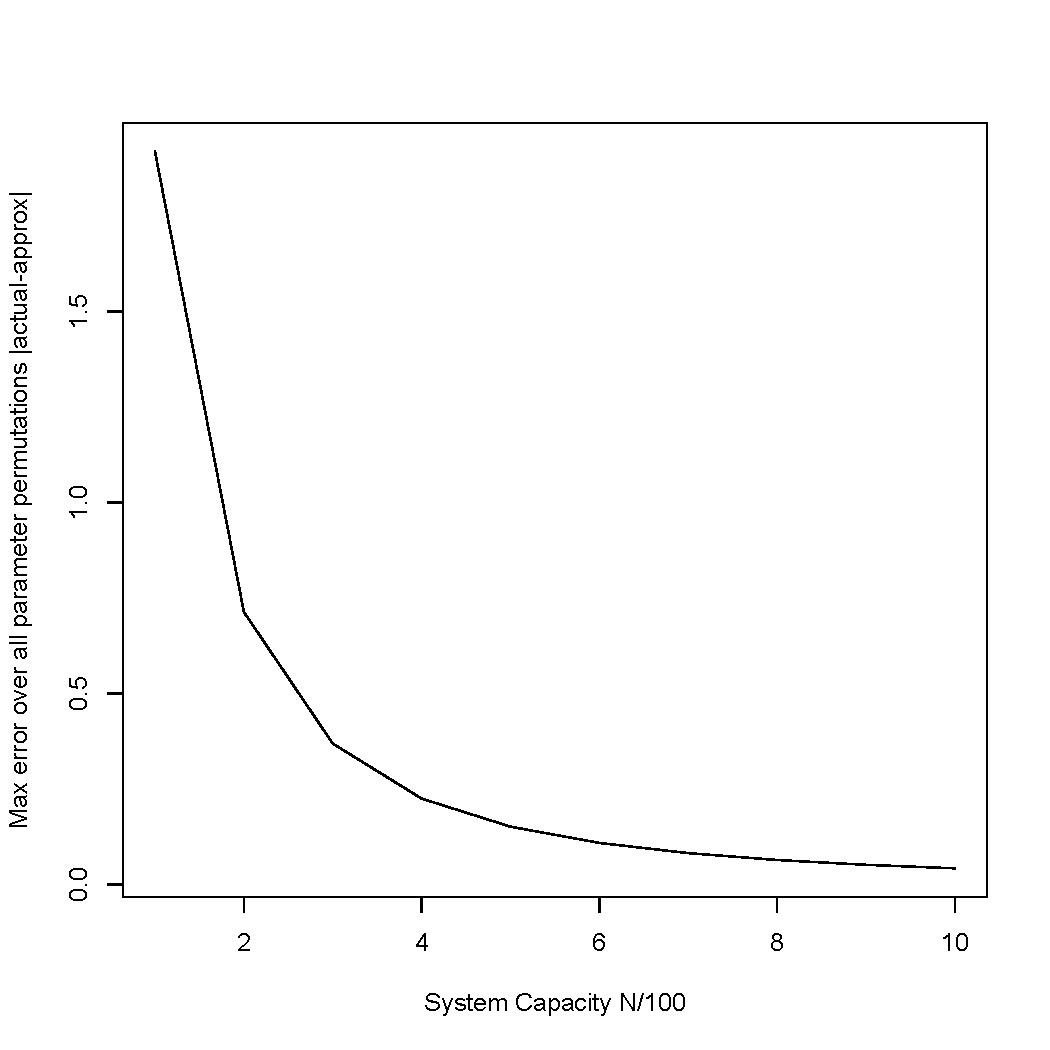
\includegraphics[width=2.5in]{FDGmaxerr.pdf} \\
  (c)&&(d)&\\
  &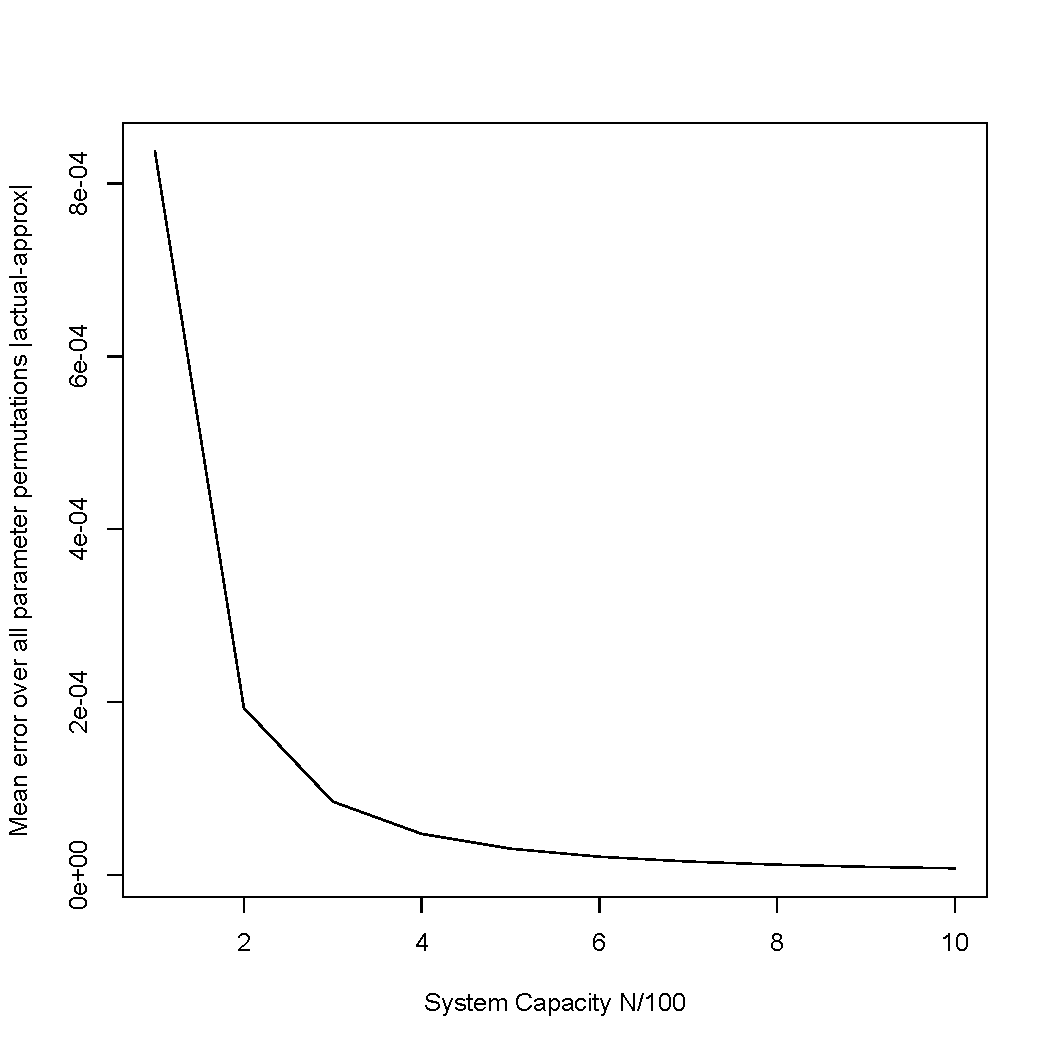
\includegraphics[width=2.5in]{FDGtmearerr.pdf} && 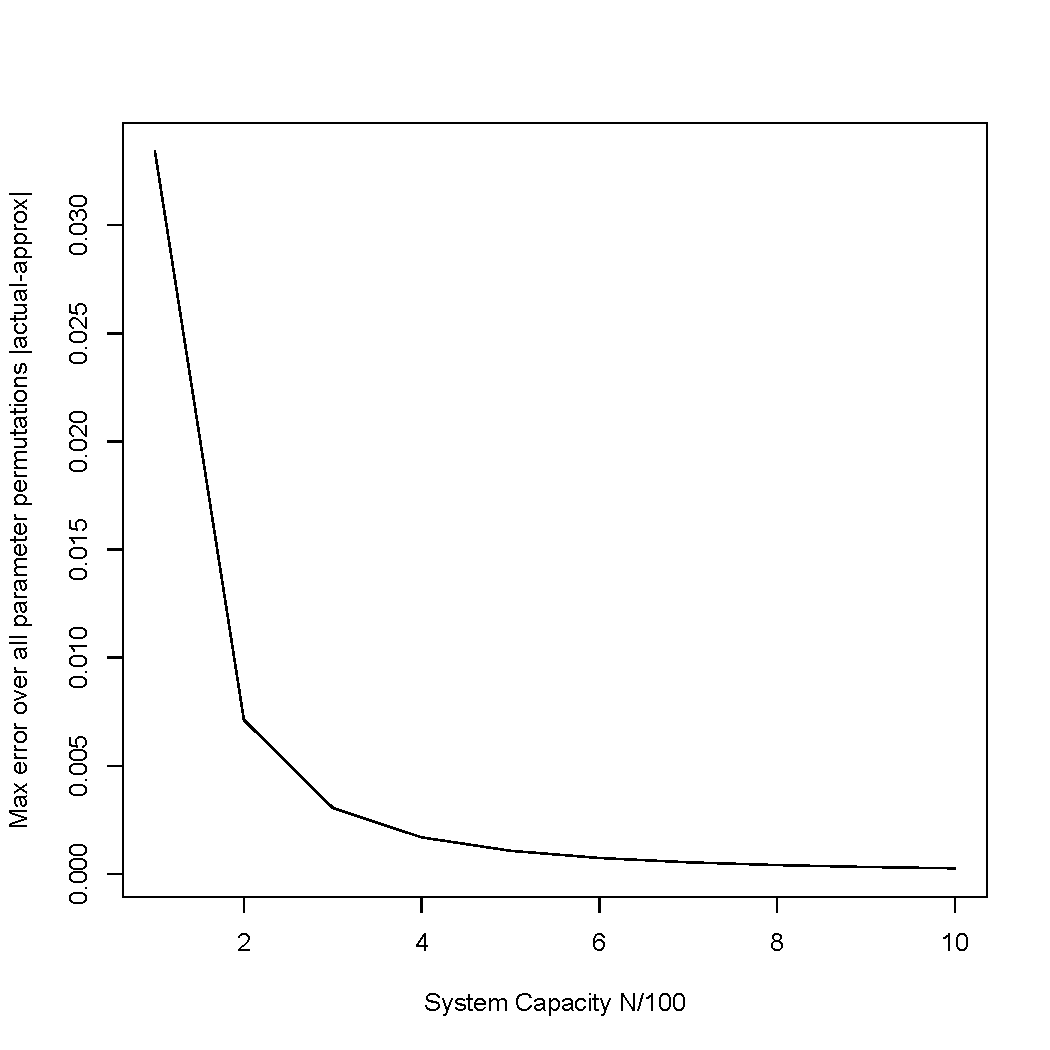
\includegraphics[width=2.5in]{FDGtmaxerr.pdf} \end{tabular}
   \caption[Errors in approximating average change: three dimensional trade-off]{\textbf{Fecundity-growth-defence trade-off:} (a-b)  How the mean (a) and maximum (b) error size at the lower boundary decrease with increased system capacity $N$. (c-d) How the mean (c) and maximum (d) error size at the upper boundary decrease with increased system capacity $N$. The error was calculated for intensities $I_1,I_2=0.1,0.2,0.3,...,0.9$ and time between disturbances $\ln(T_D)=1,2,3,...,8.$ Parameters used are $s_1=500,s_2=50,x=0.06$. Error is calculated as $| \text{AverageChangeReal}(n) - \text{AverageChange}(n) |$ for $n=1,N-1$.}
     \label{fig:fullapprox}
   \end{figure}
   
   \eappendix
   
